\documentclass{article}
\usepackage{microtype}
\usepackage{graphicx}
\usepackage{booktabs}
\usepackage{array}
\usepackage{amsmath,amssymb}
\usepackage{hyperref}
\usepackage{icml2027}
\hypersetup{pdfauthor={},pdftitle={Diagnosing Single-Robot Priority Promotion in Lifelong Warehouse Path Finding}}
\icmltitlerunning{Diagnosing Single-Robot Priority Promotion}
\begin{document}

\twocolumn[
\icmltitle{Diagnosing Single-Robot Priority Promotion in Lifelong Warehouse Path Finding\texorpdfstring{\\{\large Fixed-Reservation Checks and Validation on Public Warehouse Benchmarks}}{}}
\begin{icmlauthorlist}\icmlauthor{Anonymous Authors}{anon}\end{icmlauthorlist}
\icmlaffiliation{anon}{Anonymous Institution}
\icmlkeywords{lifelong multi-agent path finding, prioritized planning, paired replanning, service timeliness, search budget}
\vskip 0.25in]
\printAffiliationsAndNotice{}
\begin{abstract}
In warehouse planning with limited search resources per robot, moving one robot to the front of the priority order can change its access to search, its realized service, and the delays of other robots. We intervene once at the same snapshot and budget. Step-by-step replay and an independent time-layer reference establish the limits of judging service timeliness from ranks and planned actions. A separately implemented rolling safe-interval planner generates 128 source runs with sustained service and 460 paired snapshots on two Moving AI warehouse maps. Of 39 earlier focal completions, first-step direction and two-step remaining distance identify 1 and 22, respectively. In 30 cases, another robot finishes later. Across 920 focal queries, 3,680 time-layer checks verify the labels for budget, reservations, goal occupancy and window length. Earlier transfer tests on synthetic layouts included 532 pairs with recursive seeds and 720 with serial seeds under heavy stagnation. Goal-rule replay in the original planner, continuing-policy comparisons in new scenarios, and analyses of aligned tasks establish the scope of the diagnosis.
\end{abstract}
\section{Introduction}
A warehouse robot receives its next goal as soon as it reaches its current one. Classical multi-agent path finding (MAPF) starts with fixed start-goal pairs. Its lifelong variant (LMAPF) considers sustained operation with a stream of goals \citep{stern2019,ma2017,li2021}. Here, a navigation assignment counts as one task, timed from goal issuance. Online multi-agent pickup and delivery (MAPD) also includes order release, assignment, pickup, and delivery \citep{ma2017}, so its service time covers a fuller workflow.

Rolling-Horizon Collision Resolution (RHCR), by Li et al., uses continuous cross-traffic to illustrate how high throughput can coexist with individual robots remaining blocked. It monitors progress through goal visits or remaining cost \citep{li2021}. Asano et al. measure delay against an unimpeded trajectory and use counterfactual actions to distinguish when to advance or yield \citep{asano2023}. Zheng et al.'s RL-RH-PP samples fleet-wide priority orders from the same state, compares shortest-path headings with planned moves, and studies congestion recovery after a policy switch \citep[Sec.~6]{zheng2026}. For fixed goals with a total priority order, Morag et al. distinguish failure of greedy sequential planning from infeasibility under the priority constraints \citep{morag2024}.

We move one focal robot to the front once and preserve every other relative rank. The estimand is the effect of this change on realized actions and current tasks, conditional on the simulation state, initial reservations, node cap, and follow-on policy. We record search initiation, the first two executed moves, exit from the bottleneck strip, and completion for each robot. This tests whether gaining search changes the actual moves, whether changing moves speeds up service, and whether a focal gain coincides with delays for others. Local controls on fixed reservations and goal occupancy provide finer explanations. We compare what ranks and planned headings reveal on the same snapshots and verify the service clocks through independent replay. A separate planner capable of sustained operation, full public warehouse maps, and an explicit time-layer reference test these local judgments.

\section{Related Work}
\subsection{Search Scope and Evidence}
On November 18, 2026, we recorded the top seven results for each of five research queries in OpenAI's web search service. Its index covers publishers, conference proceedings, author sites, and preprints. We consolidated preprints, mirrors, and duplicates across the 35 hits by title, author, and publication identifier, leaving 16 works. We included primary studies on priority ordering, windowed completeness, passage traffic, and service timeliness. One study on free-space trajectory postprocessing and one dissertation that duplicated conference results were excluded. Targeted checks added one work each on MAPF definitions, MAPD, SIPP, and order queues, for a final set of 18. The supplement records query strings, result ranks, deduplication, and inclusion decisions. \hyperlink{display:Table1}{Table 1} identifies whether each claim was checked in the main text or the abstract. We also checked the closest methods and the provenance of the public maps against official sources or public author copies.

\subsection{Planning Mechanisms and Scope of Evidence}
Sequential planners allocate search along the current priority order. PBS branches over partial orders in response to conflicts \citep{ma2019}. PIBT inherits priorities and backtracks when making each step. Its arrival guarantee depends on conditions such as edges belonging to suitable cycles \citep{okumura2022}. Roadmap methods with safe locations rely on available retreat space and their conflict-handling rules \citep{klancar2026}. Given higher-priority reservations, SIPP compresses the feasible times for an individual robot into safe intervals \citep{phillips2011}. Local order, retreat space, and the semantics of reservations can each change the feasible set.

WinC-MAPF achieves completeness through joint heuristic updates, independent grouping, and a suitable action generator \citep{veerapaneni2025}. DAG-ECBS extends the approach to group solvers that satisfy bounded-suboptimality conditions \citep{zhang2026dag}. Real-Time LaCAM retains incremental joint search to meet its completeness conditions \citep{liang2025}. These guarantees identify when a short window can sustain progress. Our greedy per-robot replacements only require a conflict-free current window for commitment, so we track realized execution across rounds. Traffic guidance directly changes path costs and flow across aisles \citep{chen2024,zhang2024,zang2025}. Fairness in travel delay, fairness of fixed-goal paths, and order timeliness measure service at different levels \citep{asano2023,anand2026,zhang2024queue}.

\section{Model, Metrics, and Single-Round Procedure}
\subsection{Task Age and Two Service Clocks}
A robot receives a goal at time a, at an initial static shortest-path distance d. At the end of step t, a task is overdue when its relative age (t\ensuremath{-}a)/d strictly exceeds \ensuremath{\tau}. The completion step is assigned to the old task before the next one is issued. Consecutive identical goals are excluded. External zero-distance tasks can be recorded as immediate completions. Let $D_i$ be the overdue steps of robot i among N robots observed over T steps. Equation (1) gives the fleet-wide share. The main threshold is \ensuremath{\tau}=3, with sensitivity at 2 and 4. We report the median, quartiles, and maximum of per-robot shares, and the longest continuous overdue spell. A new task ends a spell. An ongoing spell at the end of measurement is right-censored. \hyperlink{display:Figure1}{Figure 1} illustrates how burden can differ at equal throughput.

\begin{equation}
F_\tau=\frac{D_1+\cdots+D_N}{NT}.
\end{equation}
Relative age includes motion, detours, and waiting. With 4 extra steps, tasks with initial distances of 1 and 10 steps have relative ages of 5 and 1.4, respectively. For initial distances of 1--8, 9--16, and 17 or more steps, we separately report the overdue share of robot-steps, absolute excess age max(t\ensuremath{-}a\ensuremath{-}d,0), and the completion share and capped P90 duration for new tasks with full 32-step follow-up.

A range of map columns defines the bottleneck strip. A robot enters the exit analysis if its current task starts and ends on opposite sides and it has yet to reach the goal side at the snapshot. F is the time to first entry, with F=0 for a robot already inside at step 0. E is the first exit to the goal side, occurring before or at completion of the current task. L is the last entry before E and is 0 when the robot starts inside and never retreats. The components F, L\ensuremath{-}F, and E\ensuremath{-}L measure time before first entry, time between first and last entry, and the final crossing. We count failures to enter separately from entries without exit. If a robot retreats, L\ensuremath{-}F includes earlier attempts and requeueing. E\ensuremath{-}L measures the last successful crossing.

The current task completes on the first visit to its goal after the snapshot. The follow-up cap is H=32. A missing completion or exit is assigned time 32, with a separate occurrence indicator. Completion at exactly step 32 counts as observed and ties an unfinished task on the capped clock. Differences are promotion minus original order, so a negative value indicates an earlier event. We retain occurrence indicators and event times per robot in each branch, and account for within-scenario dependence in robot-level summaries.

\subsection{Single Intervention}
We copy all positions, previous plans, issued goals, task indices, issue times, and the common planning seed. The treated branch only moves the focal robot to the front. The control retains the source policy order. Each branch executes its first 2 moves, then resumes the source policy from its own state until H. Goal draws are coupled by robot ID and task index. We track the task active at the snapshot for every robot. The original-order branch should reproduce the source run step by step.

Using the sampled pairs as the denominator, we report three possibly overlapping events. E1 means the focal search was skipped under the original order, starts after promotion, and leaves its executed prefix unchanged. E2 means the focal prefix changes without an earlier capped completion by H. E3 means the focal robot completes earlier on the capped clock and at least one other robot takes longer. We also count the overlap between earlier focal exit and delays to other robots. Remaining distance over the first segment measures immediate progress. In \hyperlink{display:Figure3}{Figure 3}, A retreats into r, increasing its distance to the goal from 2 to 3 while clearing the passage for B.

\subsection{Rolling Planning and Compute Accounting}
The main synthetic-layout experiment uses a planning window of W=8 and an execution prefix of 2 moves. The recursive seed orders robots by issue time and ID, assigning candidates at most one step away to build each new layer. It tries adjacent cells and waiting in order of static remaining distance. Moving takes precedence over waiting on ties, followed by cell ID. If an unclaimed destination is occupied by an unassigned robot, the procedure recursively assigns that robot's next cell. It rejects shared cells and swaps, and withdraws a failed claim before trying the next action. The selected positions form the next layer, and the process repeats 8 times. Seed construction uses only issued goals. The per-robot replacement pass then uses the tested order.


\par\medskip\noindent\begin{minipage}{\columnwidth}
\small\textbf{Algorithm 1. Plan and execute one round from a snapshot}\par\smallskip
\textbf{Input} Snapshot $S$, issued goals, tested order $\pi$, window $W$, and node cap $B$.
\begin{enumerate}\setlength{\itemsep}{1pt}\setlength{\parsep}{0pt}\setlength{\topsep}{3pt}
\item Build shared safe paths $P[1\ldots N]$. Reserve cells and reverse edges. Set $b=B$.
\item For each robot $i$ in $\pi$, remove $P[i]$ from the reservation table and log the other paths.
\item Query goal or window paths with cap $b$. Debit expanded nonterminal states.
\item Replace $P[i]$ if a candidate is returned. Otherwise retain $P[i]$.
\item Restore the occupancy and reverse edges of $P[i]$ in the table.
\item Check safety and execute two actions. Record completion and issue the next goal after each step.
\end{enumerate}
\end{minipage}\par\medskip

The low-level space-time weighted A* uses the key (t+2$d_t$, $d_t$, insertion order), where $d_t$ is the static remaining distance at the current cell. It enumerates adjacent cells in row-major order, followed by waiting, and enqueues each (cell, t) once. A goal candidate must be able to stay at its goal through the window. A path reaching the window boundary can also be submitted. A queue pop tests termination before checking the remaining budget. Once the last expansion has been charged, a subsequent terminal pop can still yield an accepted path. A query with no initial budget does not start. The budget counts expanded nonterminal space-time states. Seed construction, sorting, reservation updates, and safety checks add separate per-round work.

At each step, the robots execute the joint prefix already committed. A goal reached on step 1 is registered immediately and triggers the next goal. Step 2 still executes the committed move, and reaching the newly issued goal on that step also counts as a completion. Replanning then uses the currently issued goals. The simulator generates the task streams in advance, and each planning query sees only the goal issued at that time. The full replays include the positions, task indices, reservations of all other robots and remaining budget before each first-round query, returned candidates, and stepwise trajectories in both branches.

\subsection{Reference Models and Mechanism Controls}
For frozen tasks, joint breadth-first search (BFS) enumerates combinations of waiting and adjacent moves, excluding shared cells and swaps. Goal holding locks a robot at its first arrival. Goal release records that arrival and allows it to depart. We declare infeasibility under a given constraint model only after exhausting the reachable joint states, and classify search cutoffs as unknown. Online runs also reissue goals and execute rolling prefixes, so the frozen reference applies to the stated tasks, goal semantics, and committed actions.

The mechanism checks use sampled overdue snapshots. Within each map, fleet size, budget, and source grouping, we sort by seed and then snapshot time. For the first 3 original-order focal queries that were skipped or cut off, we hold all other reservations at query time fixed and add 32 nodes. For the first 3 pairs per stratum, we also check sequentially whether the first higher-priority candidate can be replaced. We reverse neighbor enumeration while preserving total work and arrival time or window-end distance, recheck the executed prefix for the round, and run another local query with a uniform 32-node cap. In case B, a finite time-layer search over the entire window separately compares goal holding and release. The reference minimizes first entry to the goal cell subject to a complete collision-free suffix.

\section{Scenarios, Sampling, and Policy Tests}
\subsection{Original Maps and Snapshots}
The full text and associated displays are in \hyperlink{sup:4.1}{Appendix D, Section 4.1}.

\subsection{Matched Conditions and Transfer Across Seed Constructors}
The full text and associated displays are in \hyperlink{sup:4.2}{Appendix D, Section 4.2}.

\subsection{Continuing Policies and Statistical Tests}
Seeds 2001--2016 generate 16 scenarios per map \ensuremath{\times} fleet size \ensuremath{\times} budget stratum for the continuing-policy tests. The 7 orders in \hyperlink{display:Table2}{Table 2} share starting locations, per-robot goals, seed generation, and fallback rules within each stratum. The R3 protocol recorded the protection threshold of 2.5, primary threshold of 3, candidate rules, and 5\% tolerance. R4 uses the same configuration. The added remaining-distance comparison and validation plan were fixed before the reanalysis. The 2\ensuremath{\times}2 protection experiment crosses protection on or off with congestion-based or fixed background ordering.

The primary test covers 8 strata and 2 single-rule baselines, congestion and relative age. Throughput counts completions per 100 simulation steps. We report R=mean throughput(two-stage)/mean throughput(baseline), alongside the paired absolute difference. We resample scenario seeds in pairs 50,000 times, retaining all orders for a resampled scenario. Overdue differences use percentage points. We take empirical one-sided percentile bounds with tail probability \ensuremath{\alpha}=0.05/32 and nominal confidence of 99.84375\% per bound. The 32 bounds cover 8 strata \ensuremath{\times} 2 baselines \ensuremath{\times} 2 endpoints. For each baseline, the upper bound on the overdue difference must be below 0 and the lower throughput-ratio bound above 0.95. Both baselines must pass in the same stratum. The illustrative 5\% tolerance permits 5 fewer completions per 100 baseline completions. We also report 0\% and 10\% tolerances. When a denominator is zero, we describe the absolute difference.

The exploratory 2\ensuremath{\times}2 interaction subtracts the effect of protection under fixed ordering from that under congestion ordering. We use a within-scenario difference-in-differences and report pointwise 95\% paired intervals. Remaining-distance ordering performed well descriptively in the earlier results, so we compare it using the same paired setup. Its 16 one-sided bounds form a separate family with 8 strata \ensuremath{\times} 2 endpoints and \ensuremath{\alpha}=0.05/16. We retain the unadjusted two-sided intervals.

\subsection{Public Layouts, Independent Planner, and Controls}
The public validation uses two full Moving AI warehouse maps \citep{movingai}, W1 (161\ensuremath{\times}63, 5,699 cells) and W2 (170\ensuremath{\times}84, 9,776 cells), with original obstacles and traversability. \hyperlink{display:Figure7}{Figure 7} shows the task pools. On each side of the map center we use 2 horizontal aisle rows with 23 possible start and goal cells per row. Each robot samples subsequent goals independently, with probability 0.8 of switching pools. The task stream is generated by map, fleet size, scenario seed, and per-robot task index, and is shared across the two budgets in a scenario. Each stratum uses 16 seeds, 6101--6116, 24 or 48 robots, and 240 steps with 48 for warm-up, yielding 128 source trajectories.

The independent implementation uses rolling Safe Interval Path Planning (SIPP) \citep{phillips2011}. From the issued goals it recursively builds a 10-step safe seed, with rotating tie-breaks among robots of equal age. Each query first removes that robot's own reservations. It stores the earliest arrival in each unoccupied interval of a cell, uses static remaining distance as a heuristic, and checks swaps at transitions. It can select a legal candidate that holds its goal or submit a safe path through the window. Each round shares a cap of 6N or 18N interval-state expansions and executes 2 moves. The seed constructor, reservation table, low-level search, and task advancement were implemented separately. The two planners count interval and space-time states, respectively.

The source order uses local congestion. We inspect one snapshot every 8 steps from 56 through 200. The focal robot has the largest relative age among robots that do not rank first, received their task at least 2 steps ago, did not reduce remaining distance on the preceding move, and are at static distance at most 24. We then take the first 6 moves along a deterministic static shortest path without reservations. The shared-edge label applies if another robot intends to traverse the same undirected edge in the opposite direction with an estimated entry time at most 2 steps apart. Per trajectory we randomly draw up to 2 snapshots per label. To estimate the pooled difference in proportions, we resample seeds within map and fleet size 10,000 times, keeping budgets and snapshots together in each scenario. We report a pooled interval when each group has at least 12 independent scenarios, and retain the actual denominators for sparse strata.

We make two comparisons on identical snapshots. Following Zheng et al.'s same-state sampling and direction analysis \citep[Sec.~6]{zheng2026}, each state is evaluated under the original order, focal promotion, and 6 fixed random permutations, with the same planner, seed window, and budget. A first move toward the goal scores +1, waiting 0, and moving away \ensuremath{-}1. The first criterion predicts earlier completion from a higher post-promotion direction score. The second uses shorter remaining distance after 2 moves. Both are untrained rules using observables available during planning. The service check examines every cell in all 32-step trajectories, including conflicts and goal visits, and compares the computed arrivals with the respective execution records.

We label local mechanisms using four controls. B means the actual query was skipped or cut off, and an increased cap yields a goal-holding arrival under the same reservations and window. R means no legal arrival with a continuation to the window end exists under fixed reservations, while removing other robots' reservations yields an arrival in the same window. G means allowing departure after arrival yields an earlier feasible arrival or makes an infeasible holding query feasible. W means the original window has no solution even with goal release, while extending the same reservation prefix by holding the other robots' final cells for 8 more steps yields a feasible arrival. We query each setting separately with intervals and verify the earliest arrivals and witnesses by explicit time-layer enumeration of cell, time, and arrival information. Seven small cases with predetermined labels cover individual, combined, and absent mechanisms. Local labels can overlap and apply to the stated counterfactual inputs.

We use new seeds 7101--7116 to compare two-stage ordering with longest remaining distance under the same SIPP implementation. The continuing-task metrics describe the tasks actually received and processed under each policy. The aligned cohort separately follows each robot's first task, issued at step 0 in both arms, matching robot ID, task index, and issue time for 64 steps. Throughput, overdue burden, and initial-task effects are paired by scenario within stratum, with two-sided pointwise 95\% intervals.

\section{Results}
\subsection{Fixed Goals and Feasibility}
\hyperlink{display:Table3A}{Table 3A} identifies the joint reference or legacy sequential full-plan routine in each row. The legacy routine makes all robots wait when full planning fails. \hyperlink{display:Table3B}{Table 3B} reports the actual runs of Algorithm 1. In S0, one query reaches its cap and keeps its seed, and both robots still move during the executed prefix. At W=4 and 5 in S1, the planner submits safe paths. Neither submitted full window reaches either goal. Execution is observed only for the first 2 steps. Later moves in the window are planned. The joint shortest path at W=5 is the fixed-goal reference. In S2 at cap 3, the legacy routine waits as a team. Under the same order and cap, Algorithm 1 retains each robot's seed and B arrives on step 1. Move orders, search counts, and committed and executed coordinates are included in the supplement.

\subsection{Original Pairs, Exit Times, and Cross-Robot Effects}
The full text and associated displays are in \hyperlink{sup:5.2}{Appendix D, Section 5.2}.

\subsection{Goal Occupancy in Case B and Local Mechanisms}
Of 34 eligible original-order queries that did not start or reached the cap, we select up to 3 per map \ensuremath{\times} fleet size \ensuremath{\times} cap \ensuremath{\times} source by seed and time, for 14 in total. All find a window candidate with fixed reservations and 32 additional nodes. In case B, focal robot 6 faces the same reservations from other robots, with the goal cell occupied on step 2. Independent time-layer search gives the earliest feasible arrival on step 1 with release and step 3 with holding. The original order has 0 remaining nodes and retains the seed. Promotion leaves 60 nodes and accepts a goal-holding candidate, yielding the original 1-versus-3 step outcome.

The closed-loop rerun retains the space-time A* queue key, candidate acceptance and fallback, and both orders' respective query budgets. Goal release is enabled only for the first-round focal query. A candidate that arrives and then leaves must have a legal suffix within the window, and the suffix search is charged to the same query cap. Both arms then resume the same procedure for 32 steps. Under the original order the robot completes on step 1 with either rule. Under promotion it finishes on step 3 with holding and step 1 with release. The focal queries expand 3 and 8 states, respectively. Changing the goal rule removes the 2-step delay from promotion on this snapshot.

For the same-order check, we take 45 snapshots from the 367 main pairs by the stratum rule, and 38 yield an eligible alternative. With a fixed 32-node focal cap, 2 rechecks change the candidate path and 1 changes the executed prefix. In the Single layout with 12 robots, cap 168 and raw-age source ordering at step 74 of seed 1007, robot 11 switches to a candidate that still arrives on step 6. Robot 6 changes from waiting for both moves of the prefix to arriving on step 1. This demonstrates that changing a reserved path can change execution under a fixed order. The availability and share of alternatives depend on screening and enumeration.

\subsection{Matched Conditions and Transfer Across Constructors}
The full text and associated displays are in \hyperlink{sup:5.4}{Appendix D, Section 5.4}.

\subsection{Independent Validation on Public Layouts}
All 128 source runs on the two maps have completions during the 192 measured steps, with throughput of 52.08 to 154.17 tasks per 100 steps. There are 460 sampled pairs from 2,432 scheduled snapshots. E1, E2, and E3 occur 109, 52, and 30 times. The focal robot completes in both arms in 429 pairs, the original arm alone in 2, the promoted arm alone in 7, and neither in 22. Exactly 4 original and 3 promoted focal arrivals occur at step 32 and count as completions. At least one other robot takes longer in 80 pairs, including 50 without a focal gain. The counts use the 32-step capped service clock.

There are 39 replay-verified earlier completions among 460 pairs. First-step direction alone detects 1, misses 38, and produces 2 false positives. The criterion based on remaining distance after 2 moves detects 22, misses 17, and produces 8 false positives (\hyperlink{display:Table9}{Table 9} and Figure 8a). On W1 with 24 robots and cap 144, at step 168 of seed 6106, neither observation suggests a gain for focal robot 19. The trajectory shows that it finishes 2 steps earlier while another robot finishes 1 step later. On W2 with 24 robots and cap 432, at step 136 of seed 6106, the first-step direction improves and focal robot 5 completes in 5 steps in both arms. These cases show how execution changes conclusions drawn from the same planning information.

\begin{figure*}[t]
\par\medskip\noindent\begin{minipage}{\linewidth}
\small\hypertarget{display:Table9}{}\textbf{Table 9. Planned observations and earlier completion on the same 460 snapshots}\par\smallskip
\setlength{\tabcolsep}{4pt}\renewcommand{\arraystretch}{1.12}
\begin{tabular}{@{}>{\raggedright\arraybackslash}p{\dimexpr0.25075\linewidth-2.50746\tabcolsep\relax}>{\raggedright\arraybackslash}p{\dimexpr0.11642\linewidth-1.16418\tabcolsep\relax}>{\raggedright\arraybackslash}p{\dimexpr0.11642\linewidth-1.16418\tabcolsep\relax}>{\raggedright\arraybackslash}p{\dimexpr0.11642\linewidth-1.16418\tabcolsep\relax}>{\raggedright\arraybackslash}p{\dimexpr0.15224\linewidth-1.52239\tabcolsep\relax}>{\raggedright\arraybackslash}p{\dimexpr0.24776\linewidth-2.47761\tabcolsep\relax}@{}}
\toprule
\textbf{Planning criterion} & \textbf{True +} & \textbf{False +} & \textbf{False \ensuremath{-}} & \textbf{True \ensuremath{-}} & \textbf{True + with other delay} \\
\midrule
Better first-step heading & 1 & 2 & 38 & 419 & 1 \\
Less remaining distance after two moves & 22 & 8 & 17 & 413 & 17 \\
\bottomrule
\end{tabular}
\par\smallskip The focal 32-step capped completion time decreases in 39 pairs. At least one other robot's capped time increases in 30 of those pairs.
\end{minipage}\par\medskip
\end{figure*}
Among 920 focal queries, B, R, G, and W have 59, 178, 156, and 73 positives. There are 31 queries with multiple labels. Interval searches and independent explicit enumeration agree on all 3,680 arrival checks. \hyperlink{display:Table10}{Table 10} and Figure 8b give the denominators. We group by layout, fleet size, cap, original rank, first-step vector in each arm, and each arm's change in remaining distance after 2 moves. There are 25 repeated observation signatures, of which 14 have different local labels. After also matching initial remaining distance, 2 of 4 repeated groups still have different labels. In W2 with 24 robots and cap 144, at step 168 of seed 6104 and step 176 of seed 6110, robot 5 is focal, ranks 4th, starts 1 cell from the goal, and waits through both executed prefixes. In the first snapshot an arrival witness requires removing reservations. In the second, allowing release under the same reservations changes the earliest feasible arrival from 8 steps to 1. Identical first-round observations can therefore conceal different conditions for intervention.

\begin{figure*}[t]
\par\medskip\noindent\begin{minipage}{\linewidth}\centering
\hypertarget{display:Figure8}{}%
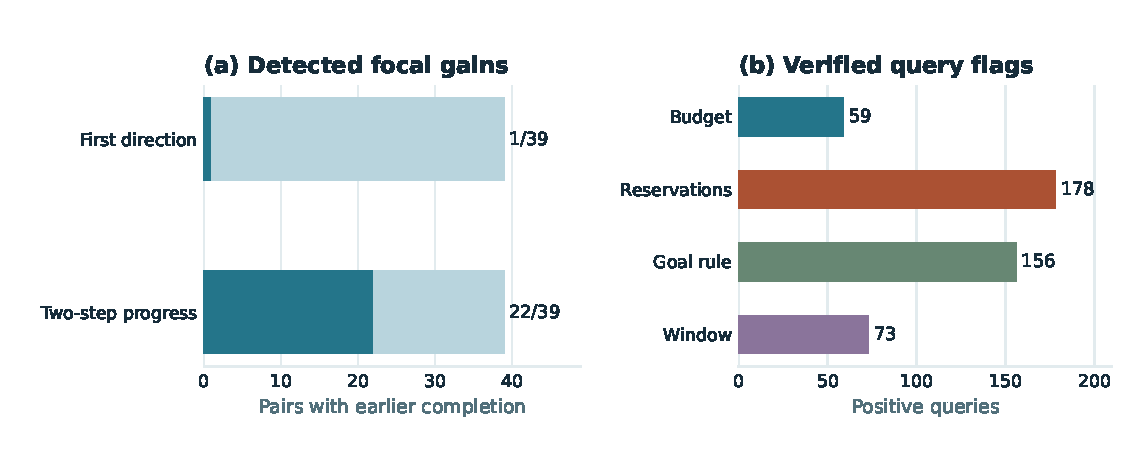
\includegraphics[width=\linewidth,height=.44\textheight,keepaspectratio]{../figures_r5/en/diagnostic_validation.pdf}\par
\small\smallskip Figure 8. Detecting earlier completion and checking local mechanisms on identical snapshots. The left panel uses 39 positives from execution paths. Table 9 gives false positives. The right panel uses 920 focal queries.
\end{minipage}\par\medskip
\end{figure*}
E3 occurs in 26/256 pairs with shared-edge intent and 4/204 without it, a difference of 8.20 percentage points (scenario interval 4.38 to 11.92). Each group covers 64 independent map \ensuremath{\times} fleet size \ensuremath{\times} seed keys. Budgets share demand and do not count as independent samples. The counts on W1 are 5/128 and 2/85, and on W2 they are 21/128 and 2/119 (\hyperlink{display:Table11}{Table 11}). In the low-budget W1 stratum with 48 robots, the group without shared edges occurs in 7 independent scenarios, and the stratum results retain those denominators. A later query-level check shows that among the 256 marked pairs, 122 original and 123 promoted cases have a corresponding opposing-edge reservation at the focal robot's estimated time. The intent marker describes potential contention. Reservations and execution determine the service outcome. The earlier proximity analysis with radius 4 used different maps, a different planner, and a different exposure definition.

Appendix \hyperlink{display:TableC1}{Table C1} gives serial per-round work and elapsed time on the same machine. Interval-state expansions are one component. Each stratum has 96 timed rounds, from building the order to finishing the joint safety check. In deployment, real-time performance also depends on execution, communication, and hardware.

\subsection{Long-Term Ordering and Joint Decision Criteria}
The seven orders account for 896 runs with 16 scenarios per stratum. \hyperlink{display:Table12}{Table 12} computes per-robot quantiles and maxima for each run, then aggregates with equal weight across strata. The longest continuous overdue spell is the average of each run's maximum across all robots and tasks. At \ensuremath{\tau}=3, the two-stage descriptive means are 75.83 completions per 100 steps and 0.58\% overdue, versus 76.95 and 0.48\% for remaining distance.

\hyperlink{display:Table13}{Table 13} gives the 16 decisions for two-stage ordering versus single-rule comparators. No adjusted upper bound on the overdue difference is below 0. For the throughput ratio, 12 lower bounds exceed 0.95. At 0\% and 10\% tolerance, 1 and 16 comparisons pass on throughput, respectively. No stratum passes the joint criterion. \hyperlink{display:Figure9}{Figure 9} shows point estimates and pointwise two-sided 95\% intervals. Decisions use the adjusted one-sided bounds in \hyperlink{display:Table13}{Table 13}. The 50,000 resamples improve numerical precision in the tails. Coverage is still limited by the small sample of 16 scenarios per stratum. Appendix B gives the full interaction results and comparison with remaining distance, which also has no passing stratum.

On Bypass with 24 robots and cap 120, the overdue shares for short tasks are 5.03\% and 8.23\% under two-stage and relative-age ordering, respectively. For medium tasks they are 0.43\% and 0.00\%, with absolute excess age of 2.70 and 2.49 steps per robot-step. Both rules have capped P90 of 32 for long tasks, with 32-step completion proportions of 89.43\% and 89.66\%. Policy-specific task turnover changes which tasks and exposed robot-steps populate each length group. The within-group percentages describe realized burden, and P90=32 reflects the 32-step follow-up limit.

The 256 new policy runs on the public maps use different seeds. Compared with remaining distance, the two-stage throughput point estimates are negative in all 8 strata. The difference in the densest W2 setting with 48 robots and cap 864 is \ensuremath{-}12.37 tasks per 100 steps (pointwise 95\% interval \ensuremath{-}14.68 to \ensuremath{-}10.19). On W1 with 48 robots and cap 288, the same 768 tasks issued at step 0 yield 470 finishes by 64 steps under two-stage and 547 under remaining distance. The difference is \ensuremath{-}10.03 percentage points (\ensuremath{-}15.76 to \ensuremath{-}4.43). Appendix \hyperlink{display:TableB3}{Table B3} includes the near-zero and wider estimates from the other strata. This experiment supplements the diagnostic study. The historical 5\% tolerance was illustrative and an operational tolerance depends on the deployment conditions.

\section{Discussion}
On matched snapshots, the two planning observables miss 38 and 17 replay-verified earlier completions, respectively. Even with matching ranks and first 2 moves, local searches can face different feasibility constraints. The independent time-layer reference makes these causes testable through fixed-input counterfactuals that increase the budget, remove reservations, change goal occupancy, or extend the window. The labels can coexist. A robot can lose a short-window opportunity due to reservations and regain feasibility in an extended window with fixed reservations. The results identify conditions that could be adjusted. Removing reservations or changing occupancy at the window boundary is a local query. Other robots' closed-loop responses require executed replay.

The case B rerun shows that changing the first focal query's goal-holding condition alters service under the same promoted order and compute cap. This case and the controlled examples provide mechanism witnesses. Operational interventions can affect later reservations, budgets, and goal issuance, so outcome sizes remain state- and implementation-dependent. The shared-edge association occurs mainly on W2, suggesting a role for alternative routes and traffic load alongside the resource definition.

The experiments cover four synthetic and two public warehouse grids, with up to 48 robots. New runs use generated demand, static four-neighbor maps, and service follow-up of at most 32 steps. The estimand concerns paired snapshots under the fixed inclusion rules. Both planners use prioritization and safe reservations. Other planning families and real order systems require their own validation. Policy results apply to the tested rules and budgets. Per-round timing describes the recorded single-machine environment.

\section{Conclusion}
Matched-state promotion and replay show whether search, execution, and service across robots change together. On public layouts with an independent planner that sustains service, replay identifies earlier completions and delays to other robots that planned directions miss. The time-layer reference checks four local mechanisms. Together, these results identify the information that the diagnostic adds. The historical joint decision criteria and the new policy runs provide no evidence of a stable service advantage for the two-stage rule.

\label{end:main}
\section*{Reproducibility Materials}
The anonymous archive contains the unmodified public maps, version checksums, frozen protocols, per-robot start and goal generators, historical and new raw logs, independent references, and Chinese and English manuscript sources. We recheck all 32 source moves in the original-order arm for the 367 historic overdue pairs and 480 historic exploratory pairs. The new runs are likewise checked step by step. The new planner was measured using Python 3.12.14 and NumPy 2.3.5 on Linux x86\_64, with script and figure tool versions documented in the supplement. Both languages use the same versioned data for the displayed tables.

\section*{AI Disclosure Statement}
ChatGPT/Codex assisted with validation design, simulator and reference code, analysis, figures, and textual revision. The reported data were produced by running the archived code and verified using independent time-layer enumeration, cell-by-cell trajectory checks, and historical replay. The authors take responsibility for the conclusions, data, and final manuscript.

\section*{Impact Statement}
Measuring realized service alongside search can help identify when a local scheduling decision delays other robots. The experiments use generated demand and discrete warehouse motion. Deployment requires validation of local safety and operational constraints.
\bibliographystyle{icml2027}
\bibliography{references}
\clearpage\onecolumn\appendix\raggedbottom
\section{Stratified Cross-Robot Delay Events}
\hyperlink{display:TableA1}{Table A1} reports 3 original-rank bands. Ratios give E3 counts divided by pair counts. Both historical cohorts use 24 robots and congestion source ordering, with different focal selection rules. The new validation applies the opposite-direction label after focal selection.

\par\medskip\noindent\begin{minipage}{\linewidth}
\small\hypertarget{display:TableA1}{}\textbf{Table A1. Stratified E3 counts at 24 robots and congestion ordering}\par\smallskip
\setlength{\tabcolsep}{4pt}\renewcommand{\arraystretch}{1.12}
\begin{tabular}{@{}>{\raggedright\arraybackslash}p{\dimexpr0.12836\linewidth-1.54030\tabcolsep\relax}>{\raggedright\arraybackslash}p{\dimexpr0.09701\linewidth-1.16418\tabcolsep\relax}>{\raggedright\arraybackslash}p{\dimexpr0.11493\linewidth-1.37910\tabcolsep\relax}>{\raggedright\arraybackslash}p{\dimexpr0.13731\linewidth-1.64776\tabcolsep\relax}>{\raggedright\arraybackslash}p{\dimexpr0.14179\linewidth-1.70149\tabcolsep\relax}>{\raggedright\arraybackslash}p{\dimexpr0.18507\linewidth-2.22090\tabcolsep\relax}>{\raggedright\arraybackslash}p{\dimexpr0.19552\linewidth-2.34627\tabcolsep\relax}@{}}
\toprule
\textbf{Layout} & \textbf{Cap} & \textbf{Rank} & \textbf{Overdue} & \textbf{Exploratory} & \textbf{New / Opposed} & \textbf{New / Unopposed} \\
\midrule
Single & 120 & 2--4 & 0/6 & 0/22 & 1/22 & 0/0 \\
Single & 120 & 5--8 & 0/7 & 1/36 & 2/41 & 0/2 \\
Single & 120 & 9+ & 0/22 & 4/62 & 2/47 & 0/13 \\
Single & 336 & 2--4 & 0/16 & 0/30 & 0/27 & 0/1 \\
Single & 336 & 5--8 & 0/5 & 1/30 & 2/32 & 0/1 \\
Single & 336 & 9+ & 0/21 & 2/60 & 1/57 & 0/7 \\
Bypass & 120 & 2--4 & 0/7 & 1/29 & 0/14 & 0/4 \\
Bypass & 120 & 5--8 & 0/2 & 0/39 & 0/18 & 0/5 \\
Bypass & 120 & 9+ & 0/11 & 7/52 & 3/37 & 3/23 \\
Bypass & 336 & 2--4 & 0/10 & 0/38 & 0/18 & 0/6 \\
Bypass & 336 & 5--8 & 0/6 & 0/27 & 0/16 & 0/6 \\
Bypass & 336 & 9+ & 0/33 & 0/55 & 0/31 & 1/17 \\
\bottomrule
\end{tabular}
\par\smallskip 0/0 indicates an empty comparison cell.
\end{minipage}\par\medskip
\par\medskip\noindent\begin{minipage}{\linewidth}
\small\hypertarget{display:TableA2}{}\textbf{Table A2. Event agreement on 532 identical snapshots under both initial seeds}\par\smallskip
\setlength{\tabcolsep}{4pt}\renewcommand{\arraystretch}{1.12}
\begin{tabular}{@{}>{\raggedright\arraybackslash}p{\dimexpr0.17164\linewidth-1.37313\tabcolsep\relax}>{\raggedright\arraybackslash}p{\dimexpr0.17463\linewidth-1.39701\tabcolsep\relax}>{\raggedright\arraybackslash}p{\dimexpr0.22388\linewidth-1.79104\tabcolsep\relax}>{\raggedright\arraybackslash}p{\dimexpr0.22388\linewidth-1.79104\tabcolsep\relax}>{\raggedright\arraybackslash}p{\dimexpr0.20597\linewidth-1.64776\tabcolsep\relax}@{}}
\toprule
\textbf{Event} & \textbf{Both} & \textbf{Recursive only} & \textbf{Serial only} & \textbf{Neither} \\
\midrule
E1 & 27 & 10 & 35 & 460 \\
E2 & 0 & 8 & 31 & 493 \\
E3 & 2 & 14 & 12 & 504 \\
\bottomrule
\end{tabular}
\par\smallskip Both arms resume recursive construction after the intervention round.
\end{minipage}\par\medskip
\par\medskip\noindent\begin{minipage}{\linewidth}
\small\hypertarget{display:TableA3}{}\textbf{Table A3. Other robots' completion status on new R4 synthetic layouts, by seed constructor}\par\smallskip
\setlength{\tabcolsep}{4pt}\renewcommand{\arraystretch}{1.12}
\begin{tabular}{@{}>{\raggedright\arraybackslash}p{\dimexpr0.13134\linewidth-1.31343\tabcolsep\relax}>{\raggedright\arraybackslash}p{\dimexpr0.11642\linewidth-1.16418\tabcolsep\relax}>{\raggedright\arraybackslash}p{\dimexpr0.13731\linewidth-1.37313\tabcolsep\relax}>{\raggedright\arraybackslash}p{\dimexpr0.22239\linewidth-2.22388\tabcolsep\relax}>{\raggedright\arraybackslash}p{\dimexpr0.14925\linewidth-1.49254\tabcolsep\relax}>{\raggedright\arraybackslash}p{\dimexpr0.24328\linewidth-2.43284\tabcolsep\relax}@{}}
\toprule
\textbf{Constructor} & \textbf{Snapshot pairs} & \textbf{Both complete} & \textbf{Original only / promoted only} & \textbf{Neither completes} & \textbf{Finish at 32, original / promoted} \\
\midrule
Recursive & 532 & 11,221 & 12 / 18 & 985 & 147 / 146 \\
Serial & 720 & 38 & 0 / 0 & 16,522 & 0 / 0 \\
\bottomrule
\end{tabular}
\par\smallskip Robot-pair counts exclude the focal robot. Focal completions in the recursive cohort are 530/532 and 529/532, respectively, and 0/720 in both serial arms.
\end{minipage}\par\medskip
\clearpage
\section{Additional Paired Policy Comparisons}
\hyperlink{display:TableB1}{Table B1} gives exploratory pointwise 95\% intervals for the 2\ensuremath{\times}2 interaction. All intervals for overdue burden cross or touch 0. \hyperlink{display:TableB2}{Table B2} gives the paired comparison to remaining-distance ordering under the same definitions, with none of the 8 strata passing the joint criterion. The archive contains the full unadjusted intervals and outputs by task-length group.

\par\medskip\noindent\begin{minipage}{\linewidth}
\small\hypertarget{display:TableB1}{}\textbf{Table B1. Interaction of protection and background order}\par\smallskip
\setlength{\tabcolsep}{4pt}\renewcommand{\arraystretch}{1.12}
\begin{tabular}{@{}>{\raggedright\arraybackslash}p{\dimexpr0.19403\linewidth-1.94030\tabcolsep\relax}>{\raggedright\arraybackslash}p{\dimexpr0.08955\linewidth-0.89552\tabcolsep\relax}>{\raggedright\arraybackslash}p{\dimexpr0.15821\linewidth-1.58209\tabcolsep\relax}>{\raggedright\arraybackslash}p{\dimexpr0.19701\linewidth-1.97015\tabcolsep\relax}>{\raggedright\arraybackslash}p{\dimexpr0.15970\linewidth-1.59701\tabcolsep\relax}>{\raggedright\arraybackslash}p{\dimexpr0.20149\linewidth-2.01493\tabcolsep\relax}@{}}
\toprule
\textbf{Layout \textperiodcentered{} N \textperiodcentered{} B} & \textbf{Seeds} & \textbf{Overdue interaction} & \textbf{95\% interval} & \textbf{Rate interaction} & \textbf{95\% interval} \\
\midrule
Single \textperiodcentered{} 12 \textperiodcentered{} 60 & 16 & +0.007 & [0.000, +0.022] & 0.000 & [0.000, 0.000] \\
Single \textperiodcentered{} 12 \textperiodcentered{} 168 & 16 & \ensuremath{-}0.004 & [\ensuremath{-}0.011, 0.000] & \ensuremath{-}0.043 & [\ensuremath{-}0.130, 0.000] \\
Single \textperiodcentered{} 24 \textperiodcentered{} 120 & 16 & \ensuremath{-}0.063 & [\ensuremath{-}0.989, +0.808] & \ensuremath{-}2.561 & [\ensuremath{-}6.380, +0.781] \\
Single \textperiodcentered{} 24 \textperiodcentered{} 336 & 16 & \ensuremath{-}0.145 & [\ensuremath{-}0.465, +0.152] & +0.477 & [\ensuremath{-}1.606, +2.821] \\
Bypass \textperiodcentered{} 12 \textperiodcentered{} 60 & 16 & +0.011 & [0.000, +0.029] & \ensuremath{-}0.043 & [\ensuremath{-}0.130, 0.000] \\
Bypass \textperiodcentered{} 12 \textperiodcentered{} 168 & 16 & 0.000 & [0.000, 0.000] & 0.000 & [0.000, 0.000] \\
Bypass \textperiodcentered{} 24 \textperiodcentered{} 120 & 16 & +0.002 & [\ensuremath{-}0.121, +0.132] & +0.608 & [\ensuremath{-}0.347, +1.519] \\
Bypass \textperiodcentered{} 24 \textperiodcentered{} 336 & 16 & \ensuremath{-}0.014 & [\ensuremath{-}0.204, +0.170] & +0.130 & [\ensuremath{-}0.911, +1.259] \\
\bottomrule
\end{tabular}
\par\smallskip Overdue units are pp, and throughput uses completions per 100 steps. Intervals are pointwise and two-sided.
\end{minipage}\par\medskip
\par\medskip\noindent\begin{minipage}{\linewidth}
\small\hypertarget{display:TableB2}{}\textbf{Table B2. Two-stage ordering versus remaining-distance ordering}\par\smallskip
\setlength{\tabcolsep}{4pt}\renewcommand{\arraystretch}{1.12}
\begin{tabular}{@{}>{\raggedright\arraybackslash}p{\dimexpr0.20448\linewidth-2.45373\tabcolsep\relax}>{\raggedright\arraybackslash}p{\dimexpr0.13134\linewidth-1.57612\tabcolsep\relax}>{\raggedright\arraybackslash}p{\dimexpr0.12687\linewidth-1.52239\tabcolsep\relax}>{\raggedright\arraybackslash}p{\dimexpr0.13433\linewidth-1.61194\tabcolsep\relax}>{\raggedright\arraybackslash}p{\dimexpr0.13881\linewidth-1.66567\tabcolsep\relax}>{\raggedright\arraybackslash}p{\dimexpr0.13881\linewidth-1.66567\tabcolsep\relax}>{\raggedright\arraybackslash}p{\dimexpr0.12537\linewidth-1.50448\tabcolsep\relax}@{}}
\toprule
\textbf{Layout \textperiodcentered{} N \textperiodcentered{} B} & \textbf{Overdue \ensuremath{\Delta}} & \textbf{Upper U} & \textbf{Rate \ensuremath{\Delta}} & \textbf{Ratio} & \textbf{Lower L} & \textbf{Pass} \\
\midrule
Single \textperiodcentered{} 12 \textperiodcentered{} 60 & \ensuremath{-}0.007 & +0.109 & \ensuremath{-}0.781 & 98.62\% & 94.16\% & No \\
Single \textperiodcentered{} 12 \textperiodcentered{} 168 & \ensuremath{-}0.029 & +0.123 & \ensuremath{-}2.170 & 96.23\% & 92.93\% & No \\
Single \textperiodcentered{} 24 \textperiodcentered{} 120 & +0.919 & +1.788 & \ensuremath{-}3.168 & 95.87\% & 90.95\% & No \\
Single \textperiodcentered{} 24 \textperiodcentered{} 336 & +0.011 & +1.063 & \ensuremath{-}0.174 & 99.77\% & 93.95\% & No \\
Bypass \textperiodcentered{} 12 \textperiodcentered{} 60 & \ensuremath{-}0.029 & +0.123 & \ensuremath{-}1.823 & 97.17\% & 95.35\% & No \\
Bypass \textperiodcentered{} 12 \textperiodcentered{} 168 & \ensuremath{-}0.116 & +0.109 & \ensuremath{-}0.391 & 99.40\% & 97.20\% & No \\
Bypass \textperiodcentered{} 24 \textperiodcentered{} 120 & +0.156 & +0.517 & \ensuremath{-}0.651 & 99.40\% & 96.56\% & No \\
Bypass \textperiodcentered{} 24 \textperiodcentered{} 336 & \ensuremath{-}0.177 & +0.092 & +0.217 & 100.19\% & 98.18\% & No \\
\bottomrule
\end{tabular}
\par\smallskip The 16 one-sided bounds form a separate family, with nominal 99.6875\% confidence per bound. Each stratum has 16 paired scenarios.
\end{minipage}\par\medskip
\par\medskip\noindent\begin{minipage}{\linewidth}
\small\hypertarget{display:TableB3}{}\textbf{Table B3. New-seed policy comparisons and aligned tasks on public layouts}\par\smallskip
\setlength{\tabcolsep}{4pt}\renewcommand{\arraystretch}{1.12}
\begin{tabular}{@{}>{\raggedright\arraybackslash}p{\dimexpr0.15522\linewidth-1.24179\tabcolsep\relax}>{\raggedright\arraybackslash}p{\dimexpr0.18060\linewidth-1.44478\tabcolsep\relax}>{\raggedright\arraybackslash}p{\dimexpr0.18209\linewidth-1.45672\tabcolsep\relax}>{\raggedright\arraybackslash}p{\dimexpr0.23134\linewidth-1.85075\tabcolsep\relax}>{\raggedright\arraybackslash}p{\dimexpr0.25075\linewidth-2.00597\tabcolsep\relax}@{}}
\toprule
\textbf{Map \textperiodcentered{} N \textperiodcentered{} cap} & \textbf{Rate change} & \textbf{Overdue change (pp)} & \textbf{Initial-task completion change (pp)} & \textbf{Capped initial-task time change (steps)} \\
\midrule
W1 \textperiodcentered{} 24 \textperiodcentered{} 144 & \ensuremath{-}2.83 [\ensuremath{-}4.43, \ensuremath{-}1.14] & +0.45 [+0.09, +0.86] & \ensuremath{-}1.56 [\ensuremath{-}4.43, +1.30] & +0.38 [\ensuremath{-}0.64, +1.40] \\
W1 \textperiodcentered{} 24 \textperiodcentered{} 432 & \ensuremath{-}1.92 [\ensuremath{-}2.90, \ensuremath{-}0.94] & +0.01 [\ensuremath{-}0.33, +0.34] & \ensuremath{-}1.82 [\ensuremath{-}4.17, 0.00] & +0.67 [\ensuremath{-}0.76, +2.10] \\
W1 \textperiodcentered{} 48 \textperiodcentered{} 288 & \ensuremath{-}11.20 [\ensuremath{-}14.58, \ensuremath{-}7.85] & +3.31 [+1.85, +4.83] & \ensuremath{-}10.03 [\ensuremath{-}15.76, \ensuremath{-}4.43] & +2.11 [+0.71, +3.62] \\
W1 \textperiodcentered{} 48 \textperiodcentered{} 864 & \ensuremath{-}0.98 [\ensuremath{-}4.04, +1.86] & +0.90 [\ensuremath{-}0.15, +1.81] & \ensuremath{-}5.47 [\ensuremath{-}11.20, +0.39] & +2.45 [+1.09, +3.88] \\
W2 \textperiodcentered{} 24 \textperiodcentered{} 144 & \ensuremath{-}1.92 [\ensuremath{-}3.91, 0.00] & \ensuremath{-}0.10 [\ensuremath{-}0.25, +0.06] & 0.00 [0.00, 0.00] & \ensuremath{-}0.29 [\ensuremath{-}1.18, +0.49] \\
W2 \textperiodcentered{} 24 \textperiodcentered{} 432 & \ensuremath{-}0.33 [\ensuremath{-}1.76, +1.14] & \ensuremath{-}0.05 [\ensuremath{-}0.22, +0.15] & 0.00 [0.00, 0.00] & +0.08 [\ensuremath{-}0.36, +0.50] \\
W2 \textperiodcentered{} 48 \textperiodcentered{} 288 & \ensuremath{-}6.05 [\ensuremath{-}8.63, \ensuremath{-}3.22] & +0.14 [\ensuremath{-}0.11, +0.40] & \ensuremath{-}0.52 [\ensuremath{-}1.56, +0.39] & +0.50 [\ensuremath{-}0.24, +1.17] \\
W2 \textperiodcentered{} 48 \textperiodcentered{} 864 & \ensuremath{-}12.37 [\ensuremath{-}14.68, \ensuremath{-}10.19] & \ensuremath{-}0.04 [\ensuremath{-}0.22, +0.16] & 0.00 [0.00, 0.00] & +1.28 [+0.65, +1.86] \\
\bottomrule
\end{tabular}
\par\smallskip Differences are two-stage minus remaining distance. Each stratum uses 16 new paired scenarios. Brackets give pointwise two-sided 95\% intervals. Both arms issue the same initial tasks at step 0, with 64 steps of follow-up.
\end{minipage}\par\medskip
\section{Measured Work and Elapsed Time}
\par\medskip\noindent\begin{minipage}{\linewidth}
\small\hypertarget{display:TableC1}{}\textbf{Table C1. End-to-end SIPP round time and workload}\par\smallskip
\setlength{\tabcolsep}{4pt}\renewcommand{\arraystretch}{1.12}
\begin{tabular}{@{}>{\raggedright\arraybackslash}p{\dimexpr0.16567\linewidth-1.65672\tabcolsep\relax}>{\raggedright\arraybackslash}p{\dimexpr0.18358\linewidth-1.83582\tabcolsep\relax}>{\raggedright\arraybackslash}p{\dimexpr0.13731\linewidth-1.37313\tabcolsep\relax}>{\raggedright\arraybackslash}p{\dimexpr0.17313\linewidth-1.73134\tabcolsep\relax}>{\raggedright\arraybackslash}p{\dimexpr0.17463\linewidth-1.74627\tabcolsep\relax}>{\raggedright\arraybackslash}p{\dimexpr0.16567\linewidth-1.65672\tabcolsep\relax}@{}}
\toprule
\textbf{Map \textperiodcentered{} N \textperiodcentered{} cap} & \textbf{Time P50 / P95 (ms)} & \textbf{Seed tests P50} & \textbf{Interval-state expansions P50} & \textbf{Neighbor-interval tests P50} & \textbf{Reservation changes P50} \\
\midrule
W1 \textperiodcentered{} 24 \textperiodcentered{} 144 & 1.81 / 2.81 & 372.5 & 144 & 619 & 1512 \\
W1 \textperiodcentered{} 24 \textperiodcentered{} 432 & 3.04 / 5.73 & 373 & 432 & 1565 & 1512 \\
W1 \textperiodcentered{} 48 \textperiodcentered{} 288 & 3.47 / 4.98 & 863 & 288 & 1218.5 & 3024 \\
W1 \textperiodcentered{} 48 \textperiodcentered{} 864 & 5.70 / 8.90 & 862 & 864 & 3179 & 3024 \\
W2 \textperiodcentered{} 24 \textperiodcentered{} 144 & 1.94 / 2.96 & 316 & 144 & 853.5 & 1512 \\
W2 \textperiodcentered{} 24 \textperiodcentered{} 432 & 3.63 / 5.36 & 309 & 432 & 2304.5 & 1512 \\
W2 \textperiodcentered{} 48 \textperiodcentered{} 288 & 3.86 / 5.87 & 760 & 288 & 1607 & 3024 \\
W2 \textperiodcentered{} 48 \textperiodcentered{} 864 & 6.66 / 9.04 & 746.5 & 864 & 4982 & 3024 \\
\bottomrule
\end{tabular}
\par\smallskip One machine runs all scenarios serially. The workload uses seed 6101 and 96 post-warm-up rounds in each stratum. Time includes sorting, seed construction, search, reservations, and validity checks.
\end{minipage}\par\medskip
\clearpage\section{Supplementary Methods, Results, and Displays}\label{app:supp}
The sections below retain their manuscript numbers so that the methods, results, and displays can be matched to the main text.
\subsection*{Section 2.1\quad Search Scope and Evidence}\hypertarget{sup:2.1}{}
\par\medskip\noindent\begin{minipage}{\linewidth}
\small\hypertarget{display:Table1}{}\textbf{Table 1. Related decisions, evidence, and source locations}\par\smallskip
\setlength{\tabcolsep}{4pt}\renewcommand{\arraystretch}{1.12}
\begin{tabular}{@{}>{\raggedright\arraybackslash}p{\dimexpr0.15224\linewidth-0.91343\tabcolsep\relax}>{\raggedright\arraybackslash}p{\dimexpr0.20896\linewidth-1.25373\tabcolsep\relax}>{\raggedright\arraybackslash}p{\dimexpr0.37164\linewidth-2.22985\tabcolsep\relax}>{\raggedright\arraybackslash}p{\dimexpr0.26716\linewidth-1.60299\tabcolsep\relax}@{}}
\toprule
\textbf{Study} & \textbf{Decision examined} & \textbf{Result or scope} & \textbf{Location checked} \\
\midrule
\citet{stern2019} & Defines conflicts, goal occupancy, and benchmarks & Separates stay at target and disappear at target, with benchmark instances and measures & Text \S{}\S{}2--3 and benchmarks \\
\citet{ma2017} & Tasks, token passing, and swaps & TP and TPTS guarantee service for well-formed pickup-and-delivery instances & Theorems 3 and 5 and experiments \\
\citet{li2021} & Rolling windows and short commitments & Cross-traffic can delay individual agents. Progress depends on the horizon and solver & Text \S{}4, example of deadlock, \S{}4.4 and Fig. 2, \S{}5 \\
\citet{asano2023} & Yielding counterfactuals and solo travel reference & Compares advancing, waiting, and realized travel delay in continuous navigation & Text pp. 888--891 (problem, delay, and filter) \\
\citet{zheng2026} & Learns and samples fleet-wide orders & Evaluates throughput and runtime, matched-state order and direction, and recovery after switching & Text \S{}\S{}5.5 and 6, Table 7 \\
\citet{phillips2011} & Safe interval compression & Known moving obstacles for a single robot, with feasible successors and search efficiency & Text theoretical analysis and experiments \\
\citet{ma2019} & Conflict-driven partial priority orders & Reports success, runtime, and cost for fixed-goal MAPF & Text PBS and experiments \\
\citet{okumura2022} & One-step inheritance and backtracking & Finite arrival under conditions including edges lying on simple cycles & Text PIBT and finite arrival conditions \\
\citet{klancar2026} & Prioritized roadmap planning with safe locations & Available safe locations are part of its completeness conditions & Publisher abstract and highlights \\
\citet{veerapaneni2025} & Grouped heuristic updates and windowed actions & Shows completeness under action-generator conditions and evaluates SS-CBS & Text WinC-MAPF, completeness, and experiments \\
\citet{zhang2026dag} & Conflict-driven group merging & Provides completeness with bounded-suboptimal group search and compares scale & Text \S{}\S{}2.4, 3, 4.1 \\
\citet{liang2025} & Real-time execution and incremental joint search & Analyzes completeness and measured success under millisecond cutoffs & Text algorithm, completeness, and experiments \\
\citet{morag2024} & Prescribed order and alternative high-priority routes & PCS is complete and optimal for PC-MAPF. Greedy failure can occur with a feasible solution under that order & Text pp. 82--84 and 88--89 \\
\citet{chen2024} & Congestion-aware guide paths & Tests traffic-flow optimization in one-shot and lifelong settings & Publisher abstract \\
\citet{zhang2024} & Optimizes guidance graph weights & Throughput for three LMAPF algorithms on eight benchmark maps & Proceedings and preprint abstracts \\
\citet{zang2025} & Online traffic guidance for PIBT & Compares adaptive, static, and hand-designed guidance & Proceedings and preprint abstracts \\
\citet{anand2026} & Fairness among fixed-goal solutions & Defines fairness with utilities or costs and evaluates search and mechanism design & Text formulation and experiments \\
\citet{zhang2024queue} & Dynamic queue priority by order due time & Examines service time and fairness for order classes & Publisher abstract and highlights \\
\bottomrule
\end{tabular}
\par\smallskip Direct text and abstract links are in literature\_evidence.tsv. The query and screening log is literature\_screening.csv.
\end{minipage}\par\medskip
\subsection*{Section 3.1\quad Task Age and Two Service Clocks}\hypertarget{sup:3.1}{}
\par\medskip\noindent\begin{minipage}{\linewidth}\centering
\hypertarget{display:Figure1}{}%
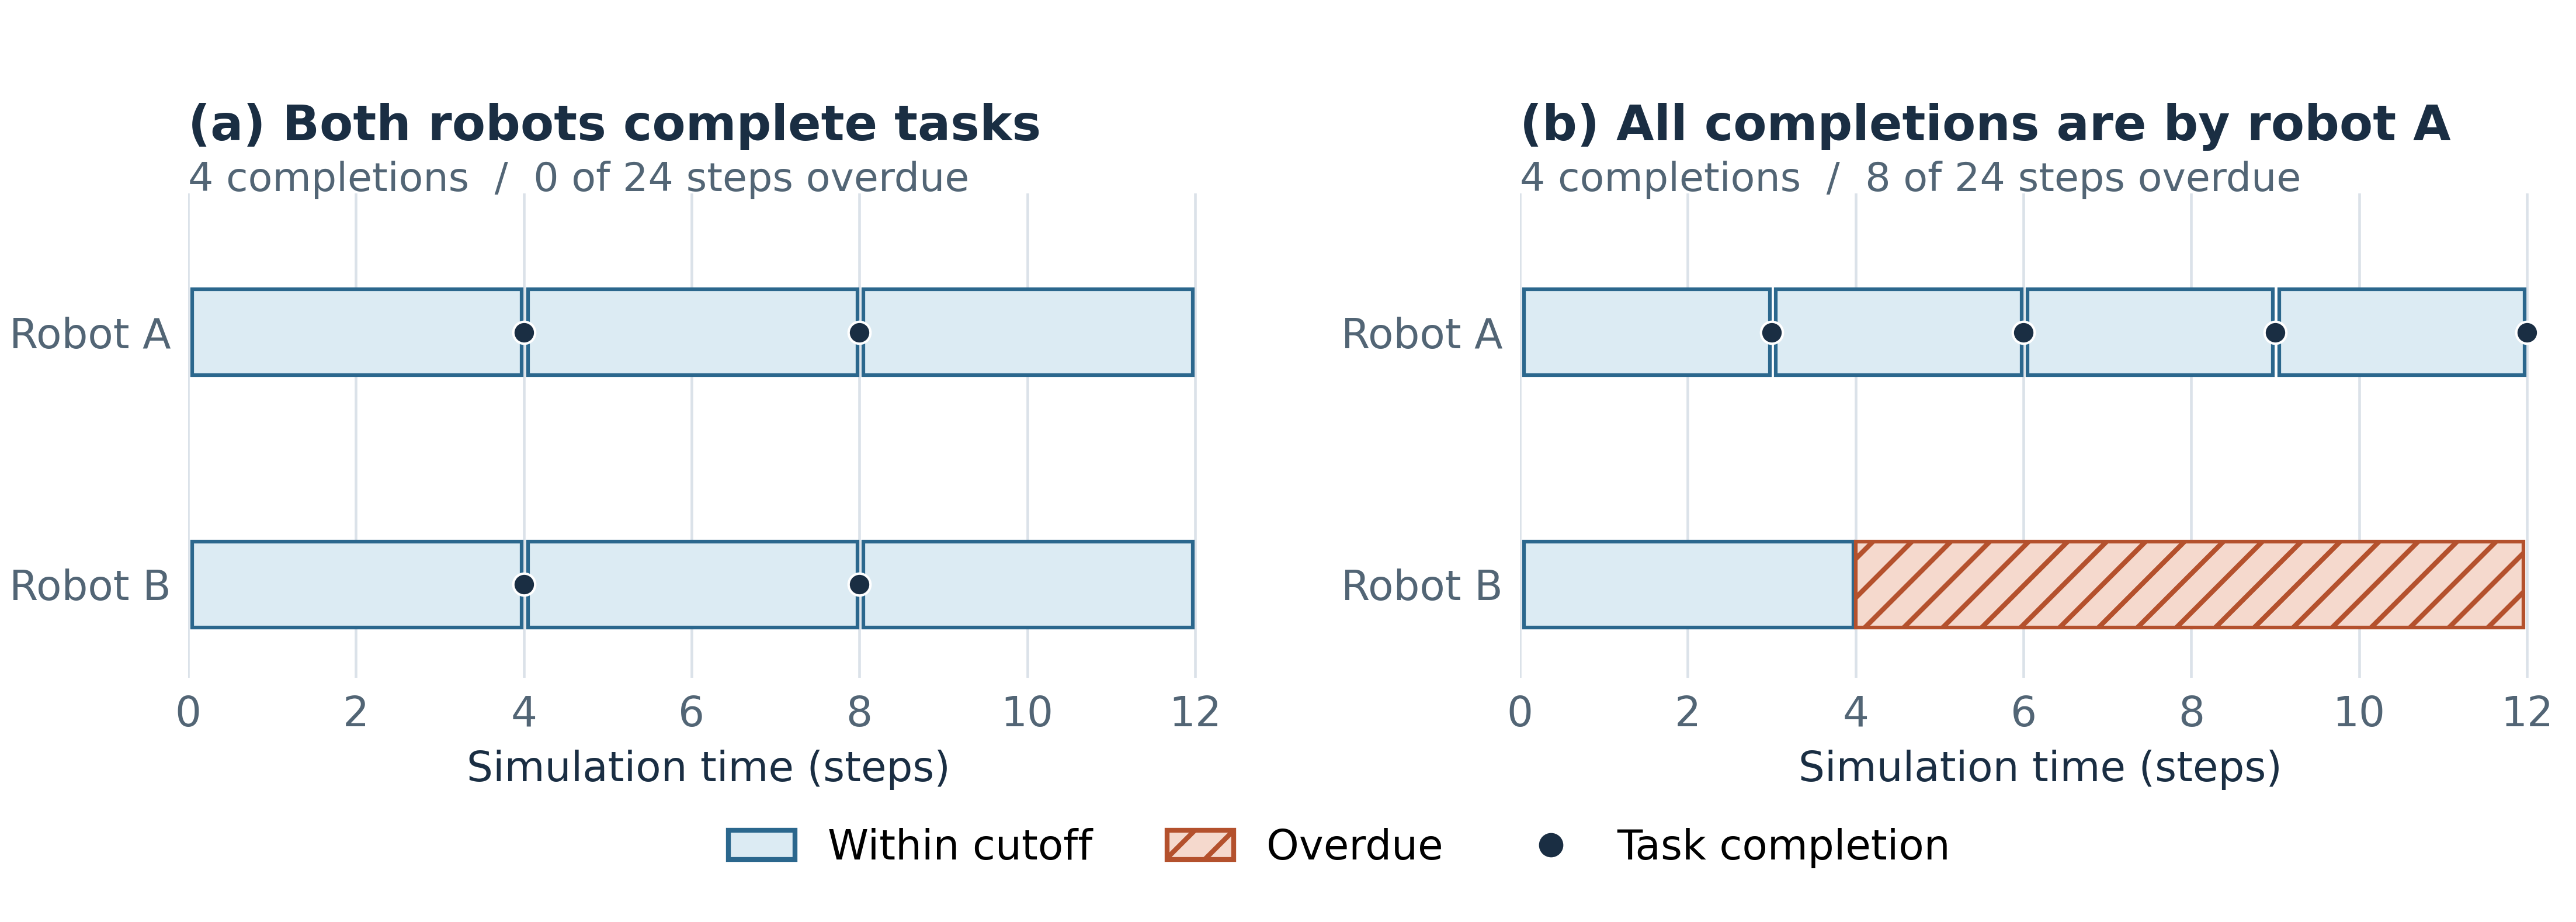
\includegraphics[width=\linewidth,height=.44\textheight,keepaspectratio]{../historical_r4/figures_en/fig1.png}\par
\small\smallskip Figure 1. Overdue robot-steps under equal throughput. Both constructed scenarios use 2 robots and 12 steps. The initial distance for every task is d=2 and the threshold is \ensuremath{\tau}=2, so an age must exceed 4 steps to count as overdue.
\end{minipage}\par\medskip
\subsection*{Section 3.2\quad Single Intervention}\hypertarget{sup:3.2}{}
\par\medskip\noindent\begin{minipage}{\linewidth}\centering
\hypertarget{display:Figure2}{}%
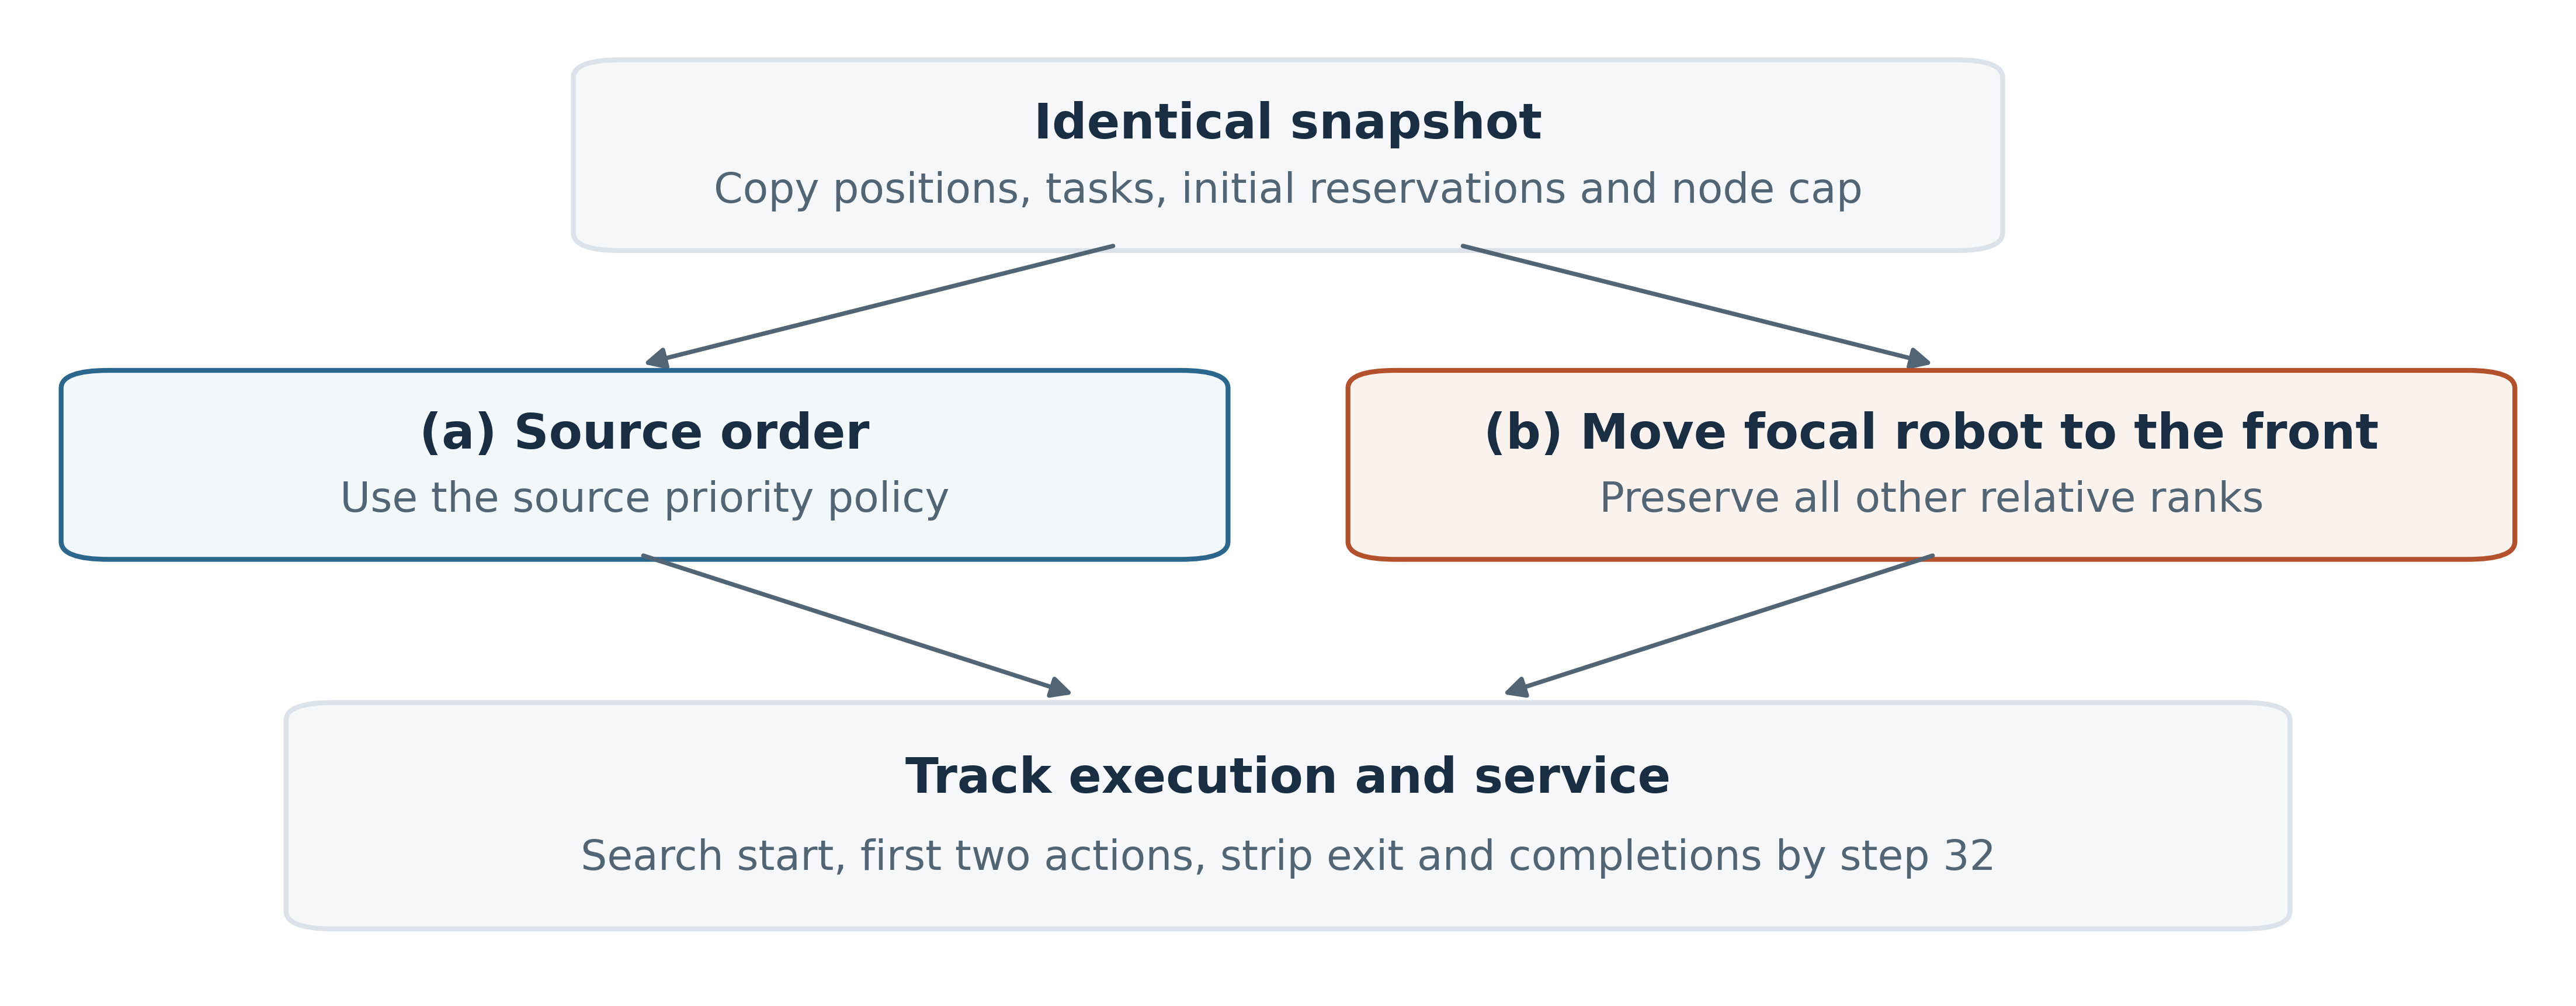
\includegraphics[width=\linewidth,height=.44\textheight,keepaspectratio]{../historical_r4/figures_en/fig2.png}\par
\small\smallskip Figure 2. One promotion and paired follow-up. Each cohort's inclusion rules specify the focal robot.
\end{minipage}\par\medskip
\par\medskip\noindent\begin{minipage}{\linewidth}\centering
\hypertarget{display:Figure3}{}%
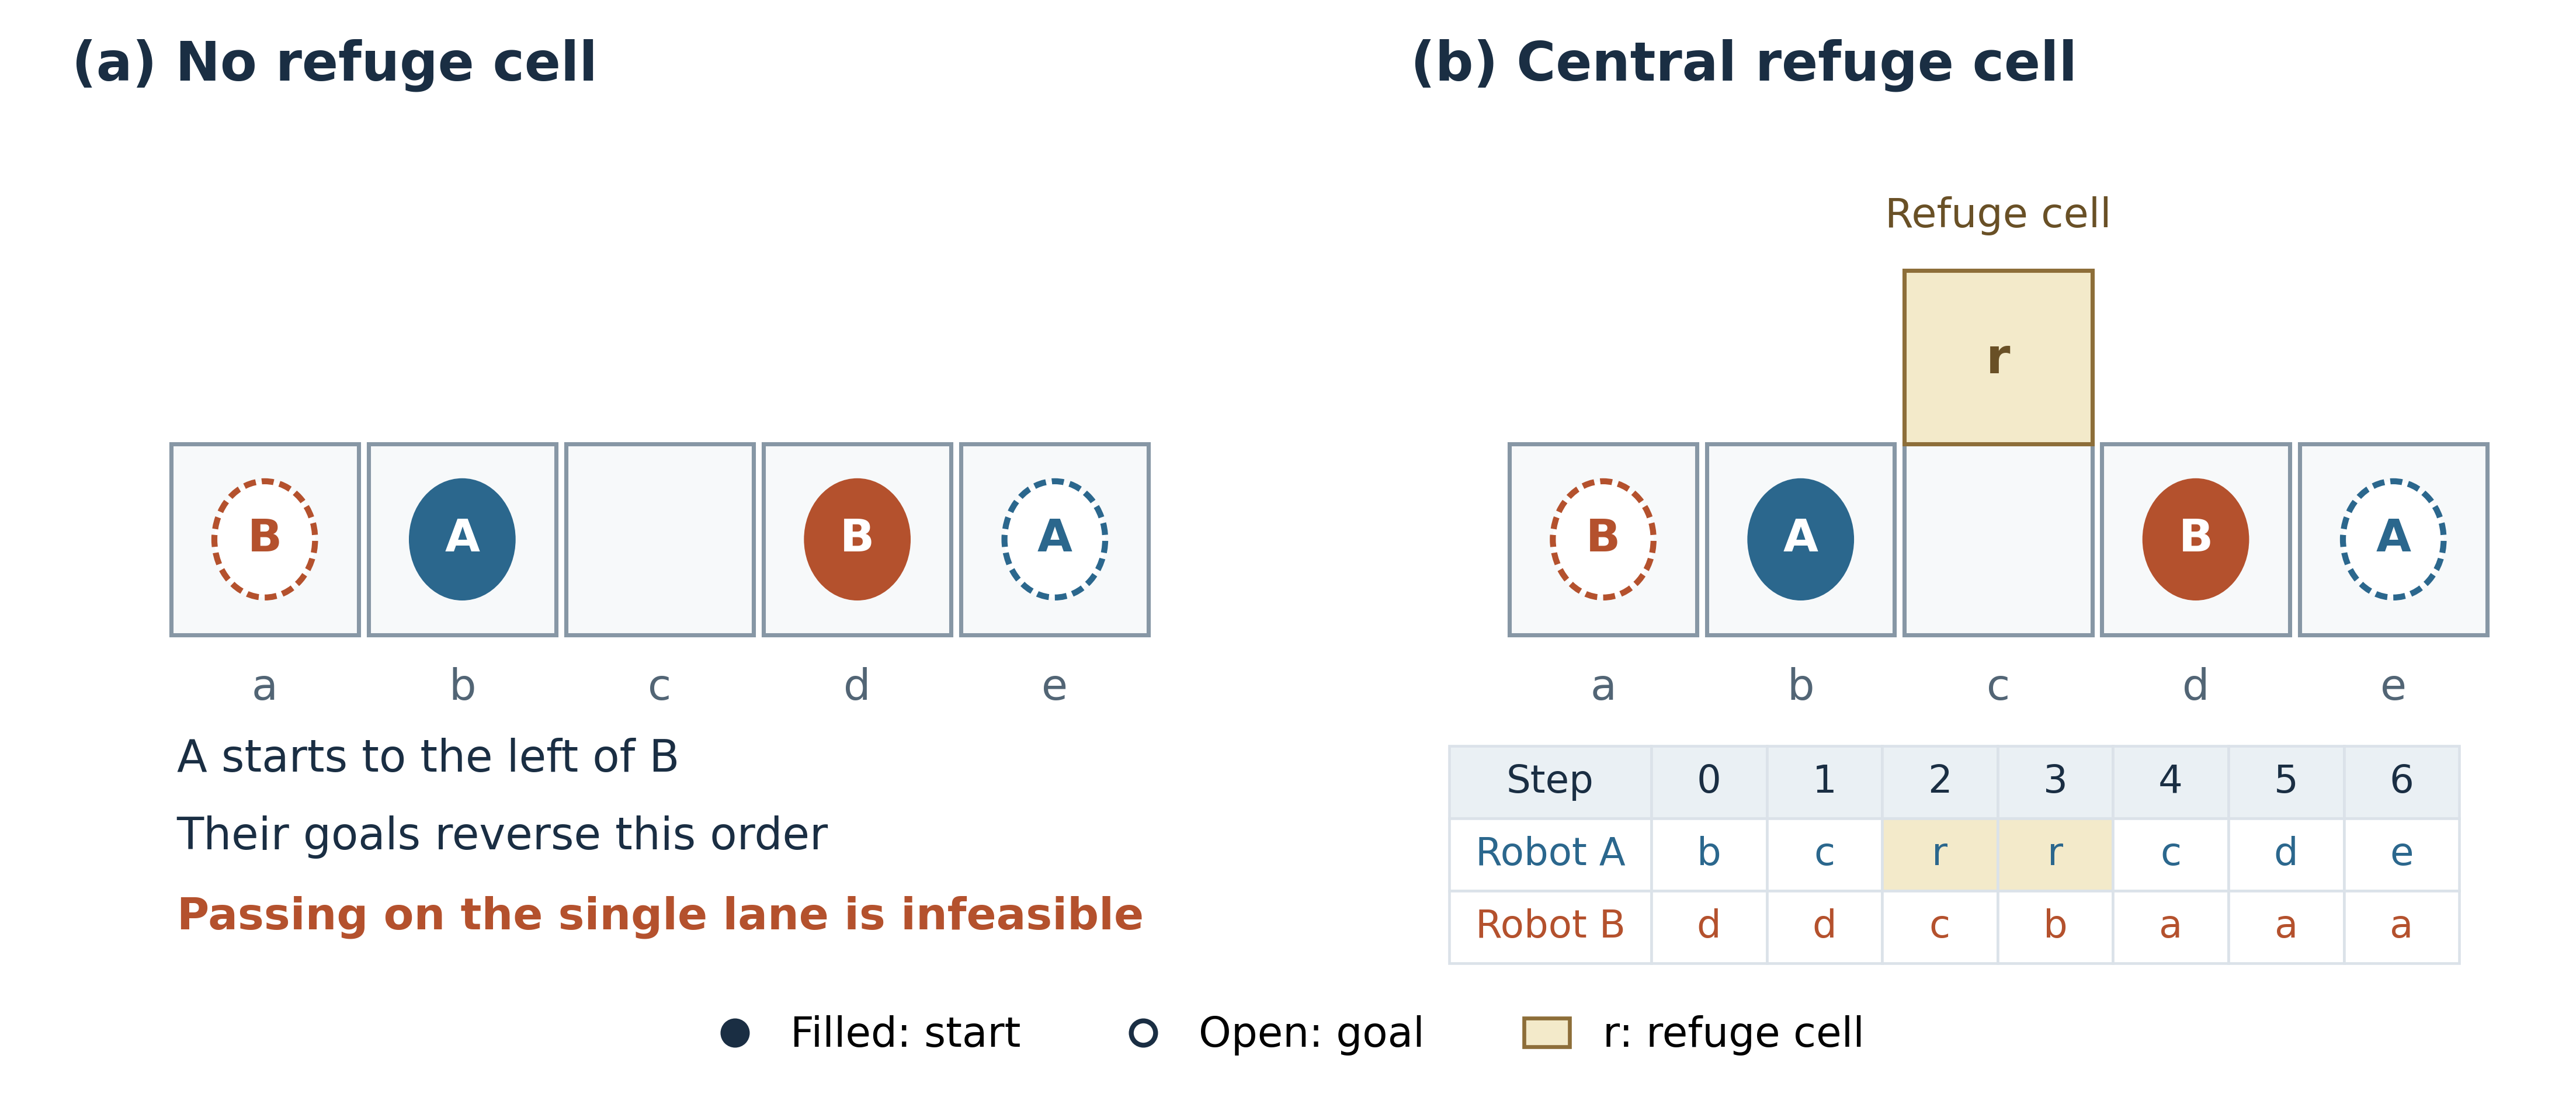
\includegraphics[width=\linewidth,height=.44\textheight,keepaspectratio]{../historical_r4/figures_en/fig3.png}\par
\small\smallskip Figure 3. A retreat cell with fixed start and goal positions. The right panel shows a verified 6-step example trajectory.
\end{minipage}\par\medskip
\subsection*{Section 4.1\quad Original Maps and Snapshots}\hypertarget{sup:4.1}{}
Two synthetic 17\ensuremath{\times}11 warehouse grids share shelf geometry and an upper perimeter passage. The Single layout has one central passage. Bypass adds a parallel passage and a connector. The bottleneck strip is x=7--9. The maps have 128 and 132 traversable cells. Fleets start with 12 or 24 robots sampled without replacement from storage areas. A subsequent goal is drawn from the opposite side with probability 0.8. Round budgets are 5N or 14N nodes. Source runs last 192 steps, with 144 steps after step 48 for policy metrics.

\par\medskip\noindent\begin{minipage}{\linewidth}\centering
\hypertarget{display:Figure4}{}%
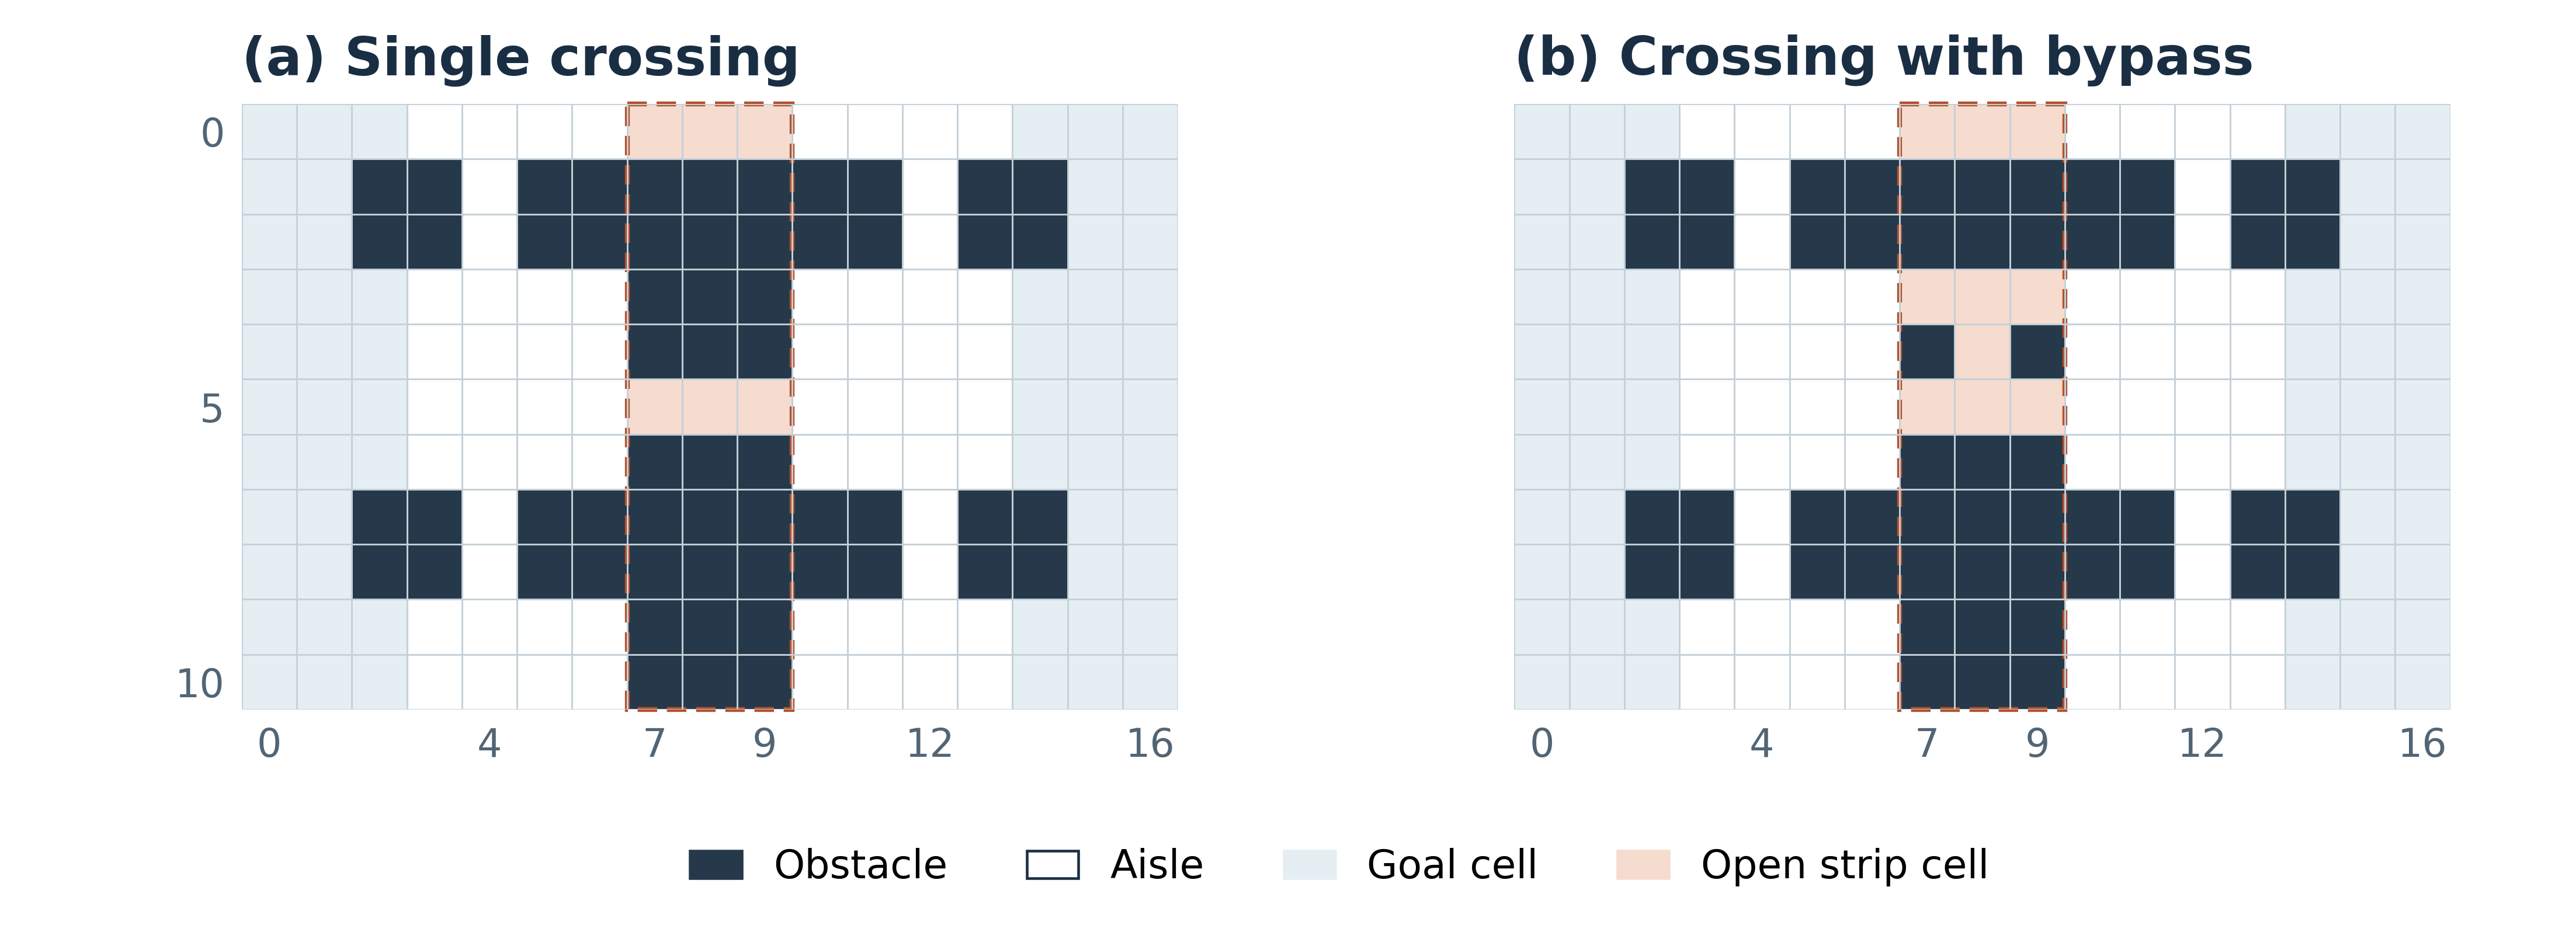
\includegraphics[width=\linewidth,height=.44\textheight,keepaspectratio]{../historical_r4/figures_en/fig4.png}\par
\small\smallskip Figure 4. Original synthetic warehouse layouts. The dashed box marks the bottleneck strip. Coordinates start at zero.
\end{minipage}\par\medskip
The source orders for the overdue cohort are raw task age and local congestion. Each map, fleet size, budget, and source uses seeds 1001--1012. For a fixed map and fleet size, starting locations and goal streams are shared across budgets and sources. At steps 48, 50, and every 2 steps through 160, we choose the robot with the highest relative age strictly above 3. Robot ID breaks ties. We discard snapshots whose focal robot already ranks first, then draw up to 5 remaining snapshots uniformly without replacement per trajectory. The average effect therefore weights the sampled snapshots, and an individual round has a smaller sampling probability on trajectories with more candidates.

The exploratory cohort was designed after inspecting overdue cases. Both maps use 24 robots, congestion ordering as the source, both budgets, and seeds 3001--3024, with up to 5 sampled snapshots per trajectory. The focal robot has the highest relative age among eligible robots, with no overdue threshold. It is on a cross-strip task at x=4--12, has yet to reach the goal side, received the task at least 2 steps ago, and failed to reduce its remaining distance on the previous move. An opposing cross-strip robot must be within Manhattan distance 4. Robots already ranked first are excluded. Scenario intervals resample seeds within map and fleet size, retaining all budgets, source orders, and snapshots for each seed.

\subsection*{Section 4.2\quad Matched Conditions and Transfer Across Seed Constructors}\hypertarget{sup:4.2}{}
Before running the added scenarios, we fixed the event definitions, candidate times, and inclusion rules. We use the original two maps, 24 robots, congestion source ordering, both budgets, and seeds 4101--4116. At steps 48, 64, and subsequent 16-step intervals through 160, we consider cross-strip robots in the near zone that have yet to reach the goal side, received the task at least 2 steps ago, and made no progress on the preceding step. The focal robot is the eligible one with the highest relative age. After selecting it, we mark whether another cross-strip robot moving in the opposite direction is within 4 cells, also in the near zone, and has yet to reach its goal side. We exclude robots already ranked first and retain all other eligible designated times. For the event E3 rate, we report the raw group difference, a sensitivity contrast stratified by map \ensuremath{\times} budget \ensuremath{\times} original rank, and scenario-resampling intervals. The marker is determined by the state, and the difference is descriptive for the selected groups.

We also generate two 21\ensuremath{\times}13 grids (\hyperlink{display:Figure6}{Figure 6}). Their strip is x=9--11 and their near zone is x=6--14. Ladder has 3 independent passages through the strip, while Offset connects staggered entrances through short vertical passages. We use seeds 5101--5112, 24 robots, both budgets, and 320-step runs. The same focal rule is applied every 16 steps from 64 through 288. The probability of each robot drawing a cross-strip goal alternates between 0.65 and 0.35 every 4 tasks, using a new random stream. Each scenario has a source trajectory from a recursive seed constructor and one from a serial constructor. At each layer, the serial procedure starts by reserving a wait for every robot. In age order, it removes the robot's own wait, chooses the safe move with smallest remaining distance, and reserves that move. It can use cells already vacated and does not recursively move unprocessed robots. Both constructors use the same replacement, goal occupancy, and execution rules.

At each eligible snapshot from a recursive source, we also copy the state and initialize both first-round branches with the serial constructor. After 2 steps both resume the recursive constructor and the source order. This compares event classifications on identical snapshots under two common seeds. For runs generated entirely by the serial or recursive constructor, we report the two inclusion counts and source throughputs separately to show how the long-run state distributions differ.

\subsection*{Section 4.3\quad Continuing Policies and Statistical Tests}\hypertarget{sup:4.3}{}
\par\medskip\noindent\begin{minipage}{\linewidth}
\small\hypertarget{display:Table2}{}\textbf{Table 2. Priority policies and factorial conditions}\par\smallskip
\setlength{\tabcolsep}{4pt}\renewcommand{\arraystretch}{1.12}
\begin{tabular}{@{}>{\raggedright\arraybackslash}p{\dimexpr0.19701\linewidth-0.78806\tabcolsep\relax}>{\raggedright\arraybackslash}p{\dimexpr0.52687\linewidth-2.10746\tabcolsep\relax}>{\raggedright\arraybackslash}p{\dimexpr0.27612\linewidth-1.10448\tabcolsep\relax}@{}}
\toprule
\textbf{Policy} & \textbf{Order} & \textbf{Role} \\
\midrule
Fixed & ID, ascending & Off / fixed \\
Raw age & Time since goal issuance, descending & Raw-age baseline \\
Relative age & Task age divided by initial shortest distance, descending & Primary comparator \\
Congestion & Count of other robots within Manhattan distance two, descending & Off / congestion, primary comparator \\
Remaining distance & Static remaining distance, descending & Secondary comparator \\
Two-stage & Relative age \textgreater{}2.5 first, ordered by relative age, then congestion & On / congestion \\
Protection + fixed & Relative age \textgreater{}2.5 first, ordered by relative age, then ID & On / fixed \\
\bottomrule
\end{tabular}
\par\smallskip Robot ID breaks all ties. The protection cutoff is 2.5, and the primary evaluation cutoff is 3.
\end{minipage}\par\medskip
\subsection*{Section 4.4\quad Public Layouts, Independent Planner, and Controls}\hypertarget{sup:4.4}{}
\par\medskip\noindent\begin{minipage}{\linewidth}\centering
\hypertarget{display:Figure7}{}%
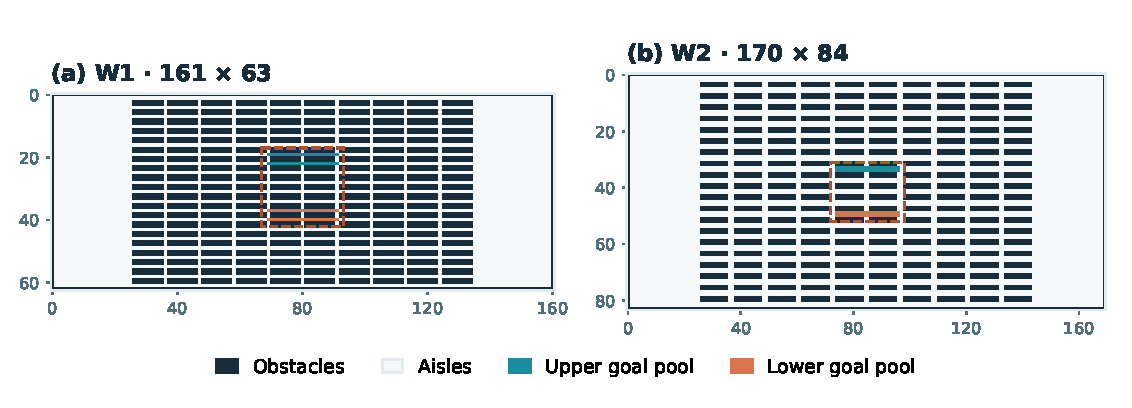
\includegraphics[width=\linewidth,height=.44\textheight,keepaspectratio]{../figures_r5/en/public_layout.pdf}\par
\small\smallskip Figure 7. Moving AI warehouse maps and locations of generated tasks. Dashed boxes mark the task-pool regions. Routing uses the complete layouts with the original obstacles.
\end{minipage}\par\medskip
\subsection*{Section 5.1\quad Fixed Goals and Feasibility}\hypertarget{sup:5.1}{}
\par\medskip\noindent\begin{minipage}{\linewidth}
\small\hypertarget{display:Table3A}{}\textbf{Table 3A. Joint reference and legacy sequential planning for fixed goals}\par\smallskip
\setlength{\tabcolsep}{4pt}\renewcommand{\arraystretch}{1.12}
\begin{tabular}{@{}>{\raggedright\arraybackslash}p{\dimexpr0.10149\linewidth-0.60896\tabcolsep\relax}>{\raggedright\arraybackslash}p{\dimexpr0.21791\linewidth-1.30746\tabcolsep\relax}>{\raggedright\arraybackslash}p{\dimexpr0.27612\linewidth-1.65672\tabcolsep\relax}>{\raggedright\arraybackslash}p{\dimexpr0.40448\linewidth-2.42687\tabcolsep\relax}@{}}
\toprule
\textbf{Case} & \textbf{Output source} & \textbf{Conditions} & \textbf{Finding or witness} \\
\midrule
S0 & Joint BFS & Five-cell line, hold at first arrival & Exhausts 10 configurations with no joint fixed-goal solution. \\
S0 & Legacy sequential full plan & A first, cap 20 & No complete joint plan found. The team waits. \\
S1 & Joint BFS & Retreat cell, depth 4 / 5 & Depth 4 cannot complete both tasks, with 20 expansions. Depth 5 finds a shortest solution with 29 expansions. \\
S2 & Joint BFS & Six-cell 2D grid, hold at first arrival & Completion in 3 steps with 15 expansions. \\
S2 & Legacy sequential full plan & A first, cap 20 & A's first shortest route blocks B. The team waits. Another equally long route yields a solution. \\
S2 & Legacy sequential full plan & B first, cap 3 / 20 & At cap 3 the routine cuts off and the team waits. At cap 20 it commits a 3-step plan. \\
S3 & Joint BFS & Four-cell T, hold / release & Goal holding exhausts 5 states. Release gives a 3-step witness. \\
\bottomrule
\end{tabular}
\par\smallskip The legacy routine makes the full team wait when full planning fails. The joint reference establishes feasibility for frozen goals under the indicated goal semantics.
\end{minipage}\par\medskip
\par\medskip\noindent\begin{minipage}{\linewidth}
\small\hypertarget{display:Table3B}{}\textbf{Table 3B. First-round commitment and execution in Algorithm 1}\par\smallskip
\setlength{\tabcolsep}{4pt}\renewcommand{\arraystretch}{1.12}
\begin{tabular}{@{}>{\raggedright\arraybackslash}p{\dimexpr0.08060\linewidth-1.12836\tabcolsep\relax}>{\raggedright\arraybackslash}p{\dimexpr0.10746\linewidth-1.50448\tabcolsep\relax}>{\raggedright\arraybackslash}p{\dimexpr0.08806\linewidth-1.23284\tabcolsep\relax}>{\raggedright\arraybackslash}p{\dimexpr0.10299\linewidth-1.44179\tabcolsep\relax}>{\raggedright\arraybackslash}p{\dimexpr0.22388\linewidth-3.13433\tabcolsep\relax}>{\raggedright\arraybackslash}p{\dimexpr0.10448\linewidth-1.46269\tabcolsep\relax}>{\raggedright\arraybackslash}p{\dimexpr0.14328\linewidth-2.00597\tabcolsep\relax}>{\raggedright\arraybackslash}p{\dimexpr0.14925\linewidth-2.08955\tabcolsep\relax}@{}}
\toprule
\textbf{Case} & \textbf{Window W} & \textbf{Cap} & \textbf{Order} & \textbf{Queries A / B} & \textbf{Fallbacks} & \textbf{Goal hits in plan} & \textbf{Hits in 2 moves} \\
\midrule
S0 & 8 & 20 & A\ensuremath{\rightarrow}B & Window / Cutoff & 1 & --- / --- & --- / --- \\
S1 & 4 & 32 & A\ensuremath{\rightarrow}B & Window / Window & 0 & --- / --- & --- / --- \\
S1 & 5 & 32 & A\ensuremath{\rightarrow}B & Window / Window & 0 & --- / --- & --- / --- \\
S2 & 8 & 20 & A\ensuremath{\rightarrow}B & Goal / Exhausted & 1 & 3 / 1 & --- / 1 \\
S2 & 8 & 3 & B\ensuremath{\rightarrow}A & Cutoff / Exhausted & 2 & 3 / 1 & --- / 1 \\
S2 & 8 & 20 & B\ensuremath{\rightarrow}A & Goal / Exhausted & 1 & 3 / 1 & --- / 1 \\
S3 & 8 & 20 & A\ensuremath{\rightarrow}B & Goal / Window & 0 & 1 / --- & 1 / --- \\
\bottomrule
\end{tabular}
\par\smallskip Each robot with no returned candidate retains its safe seed. Arrival columns list A then B. Dashes indicate that no goal is reached in the observation window for that column.
\end{minipage}\par\medskip
\subsection*{Section 5.2\quad Original Pairs, Exit Times, and Cross-Robot Effects}\hypertarget{sup:5.2}{}
\par\medskip\noindent\begin{minipage}{\linewidth}
\small\hypertarget{display:Table4}{}\textbf{Table 4. Snapshot selection in the original cohorts}\par\smallskip
\setlength{\tabcolsep}{4pt}\renewcommand{\arraystretch}{1.12}
\begin{tabular}{@{}>{\raggedright\arraybackslash}p{\dimexpr0.22687\linewidth-2.72239\tabcolsep\relax}>{\raggedright\arraybackslash}p{\dimexpr0.18209\linewidth-2.18507\tabcolsep\relax}>{\raggedright\arraybackslash}p{\dimexpr0.12239\linewidth-1.46866\tabcolsep\relax}>{\raggedright\arraybackslash}p{\dimexpr0.09254\linewidth-1.11045\tabcolsep\relax}>{\raggedright\arraybackslash}p{\dimexpr0.11194\linewidth-1.34328\tabcolsep\relax}>{\raggedright\arraybackslash}p{\dimexpr0.11045\linewidth-1.32537\tabcolsep\relax}>{\raggedright\arraybackslash}p{\dimexpr0.15373\linewidth-1.84478\tabcolsep\relax}@{}}
\toprule
\textbf{Cohort} & \textbf{Runs (contributing)} & \textbf{Ticks} & \textbf{Trigger} & \textbf{Already first} & \textbf{Eligible} & \textbf{Sampled} \\
\midrule
Overdue / raw age & 96 (51) & 5,472 & 567 & 195 & 372 & 191 \\
Overdue / congestion & 96 (51) & 5,472 & 343 & 12 & 331 & 176 \\
Exploratory & 96 (96) & 5,472 & 4,621 & 280 & 4,341 & 480 \\
\bottomrule
\end{tabular}

\end{minipage}\par\medskip
Of 10,944 planning rounds in the primary cohort, 910 trigger overdue screening and 207 have the focal robot already first. The 703 eligible rounds yield 367 sampled pairs from 102 trajectories. In \hyperlink{display:Table5}{Table 5}, 26/30 new search opportunities leave the focal prefix unchanged and none of the 12/12 changed prefixes lead to earlier completion. In each arm, 146 pairs have at least one skipped or truncated query in the first round. The focal queries fall back to the seed with no candidate 37 and 4 times, return the exact seed as a candidate 248 and 275 times, commit the seed's full window 285 and 279 times, and execute its first 2 moves 297 and 291 times, respectively. All 367 focal robots finish by step 32 in both arms. One finishes earlier and 10 later, with mean difference +0.12 steps (95\% interval 0.03 to 0.24). Exit time is identical for all 51 eligible cross-strip focal pairs.

\par\medskip\noindent\begin{minipage}{\linewidth}
\small\hypertarget{display:Table5}{}\textbf{Table 5. First-round actions and 32-step service events}\par\smallskip
\setlength{\tabcolsep}{4pt}\renewcommand{\arraystretch}{1.12}
\begin{tabular}{@{}>{\raggedright\arraybackslash}p{\dimexpr0.17612\linewidth-2.46567\tabcolsep\relax}>{\raggedright\arraybackslash}p{\dimexpr0.07463\linewidth-1.04478\tabcolsep\relax}>{\raggedright\arraybackslash}p{\dimexpr0.05224\linewidth-0.73134\tabcolsep\relax}>{\raggedright\arraybackslash}p{\dimexpr0.05224\linewidth-0.73134\tabcolsep\relax}>{\raggedright\arraybackslash}p{\dimexpr0.05224\linewidth-0.73134\tabcolsep\relax}>{\raggedright\arraybackslash}p{\dimexpr0.10746\linewidth-1.50448\tabcolsep\relax}>{\raggedright\arraybackslash}p{\dimexpr0.24179\linewidth-3.38507\tabcolsep\relax}>{\raggedright\arraybackslash}p{\dimexpr0.24328\linewidth-3.40597\tabcolsep\relax}@{}}
\toprule
\textbf{Cohort} & \textbf{Pairs} & \textbf{E1} & \textbf{E2} & \textbf{E3} & \textbf{Exit n} & \textbf{Completion \ensuremath{\Delta} (steps)} & \textbf{Exit \ensuremath{\Delta} (steps)} \\
\midrule
Overdue / raw age & 191 & 3 & 3 & 0 & 37 & +0.047 [0.000, +0.144] & 0.000 [0.000, 0.000] \\
Overdue / congestion & 176 & 23 & 9 & 0 & 14 & +0.193 [+0.023, +0.430] & 0.000 [0.000, 0.000] \\
Exploratory & 480 & 43 & 10 & 16 & 480 & \ensuremath{-}0.119 [\ensuremath{-}0.208, \ensuremath{-}0.048] & \ensuremath{-}0.121 [\ensuremath{-}0.210, \ensuremath{-}0.046] \\
\bottomrule
\end{tabular}
\par\smallskip Differences are promoted minus original. Brackets are two-sided 95\% scenario-bootstrap intervals. See \S{}3.2 for events.
\end{minipage}\par\medskip
All 480 exploratory focal robots exit the strip in both arms. \hyperlink{display:Table6}{Table 6} gives common denominators for F, L\ensuremath{-}F, and E\ensuremath{-}L. There are 328 robots outside at step 0, and in each arm 26 retreat and reenter. Exit times sum to 3,028 and 2,982 steps for outside starts, and to 1,291 and 1,279 for inside starts, in the original and promoted arms. Adding the totals and dividing by 480 gives 8.9979 and 8.8771 steps, respectively. For outside starts, first entry averages 0.16 steps earlier and the last two components increase by about 0.02 steps in total. For inside starts, remaining exit time decreases by 0.08 steps.

\par\medskip\noindent\begin{minipage}{\linewidth}
\small\hypertarget{display:Table6}{}\textbf{Table 6. Reconstruction of exploratory exit times}\par\smallskip
\setlength{\tabcolsep}{4pt}\renewcommand{\arraystretch}{1.12}
\begin{tabular}{@{}>{\raggedright\arraybackslash}p{\dimexpr0.12985\linewidth-1.81791\tabcolsep\relax}>{\raggedright\arraybackslash}p{\dimexpr0.13881\linewidth-1.94328\tabcolsep\relax}>{\raggedright\arraybackslash}p{\dimexpr0.08955\linewidth-1.25373\tabcolsep\relax}>{\raggedright\arraybackslash}p{\dimexpr0.11194\linewidth-1.56716\tabcolsep\relax}>{\raggedright\arraybackslash}p{\dimexpr0.12687\linewidth-1.77612\tabcolsep\relax}>{\raggedright\arraybackslash}p{\dimexpr0.12687\linewidth-1.77612\tabcolsep\relax}>{\raggedright\arraybackslash}p{\dimexpr0.13284\linewidth-1.85970\tabcolsep\relax}>{\raggedright\arraybackslash}p{\dimexpr0.14328\linewidth-2.00597\tabcolsep\relax}@{}}
\toprule
\textbf{Arm} & \textbf{Start} & \textbf{n} & \textbf{F} & \textbf{L \ensuremath{-} F} & \textbf{E \ensuremath{-} L} & \textbf{Mean E} & \textbf{Total E steps} \\
\midrule
Original & Outside & 328 & 5.1860 & 0.8201 & 3.2256 & 9.2317 & 3,028 \\
Original & Inside & 152 & 0.0000 & 5.3026 & 3.1908 & 8.4934 & 1,291 \\
Original & All & 480 & 3.5438 & 2.2396 & 3.2146 & 8.9979 & 4,319 \\
Promoted & Outside & 328 & 5.0244 & 0.8354 & 3.2317 & 9.0915 & 2,982 \\
Promoted & Inside & 152 & 0.0000 & 5.2303 & 3.1842 & 8.4145 & 1,279 \\
Promoted & All & 480 & 3.4333 & 2.2271 & 3.2167 & 8.8771 & 4,261 \\
\bottomrule
\end{tabular}
\par\smallskip Units are steps. In each arm, 26 outside starts and 84 inside starts retreat to the origin bank at least once.
\end{minipage}\par\medskip
The sum of focal exit-time differences is \ensuremath{-}58 steps and that of current-task completion differences is \ensuremath{-}57. The two differences disagree in 4 pairs. The separately resampled 95\% intervals agree to 2 decimals, and \hyperlink{display:Table5}{Table 5} reports 3 decimals to distinguish them. The mean capped time falls in the exploratory cohort, while completion by step 32 declines from 479/480 to 478/480. Both arms finish in 478 pairs, only the original in 1, and neither in 1. Event E3 in \hyperlink{display:Table5}{Table 5} uses earlier completion (16 cases). Substituting earlier exit yields 17.

\hyperlink{display:Table7}{Table 7} reports results for robots other than the focal one. In 30 exploratory pairs at least one other robot takes longer, including 14 in which the focal robot does not finish earlier. At least 2 other robots take longer in 19 pairs. The 81 positive time differences have a median of 3 steps, P90 of 11, and maximum of 23. Completion status and finishes at exactly step 32 are reported per robot. Two unfinished branches contribute a zero capped difference. A one-arm completion can tie the other arm if it occurs exactly at the cap. Scenario and per-robot records are supplied in the supplement.

\par\medskip\noindent\begin{minipage}{\linewidth}
\small\hypertarget{display:Table7}{}\textbf{Table 7. Capped completion-time differences and completion status of other robots by step 32}\par\smallskip
\setlength{\tabcolsep}{4pt}\renewcommand{\arraystretch}{1.12}
\begin{tabular}{@{}>{\raggedright\arraybackslash}p{\dimexpr0.32239\linewidth-2.57910\tabcolsep\relax}>{\raggedright\arraybackslash}p{\dimexpr0.16269\linewidth-1.30149\tabcolsep\relax}>{\raggedright\arraybackslash}p{\dimexpr0.16716\linewidth-1.33731\tabcolsep\relax}>{\raggedright\arraybackslash}p{\dimexpr0.17463\linewidth-1.39701\tabcolsep\relax}>{\raggedright\arraybackslash}p{\dimexpr0.17313\linewidth-1.38507\tabcolsep\relax}@{}}
\toprule
\textbf{Measure} & \textbf{Overdue} & \textbf{Exploratory} & \textbf{Matched conditions} & \textbf{New layouts} \\
\midrule
Snapshot pairs & 367 & 480 & 445 & 1,252 \\
Pairs with any delay elsewhere & 10 & 30 & 27 & 26 \\
Pairs with \ensuremath{\geq}2 delayed other robots & 8 & 19 & 19 & 19 \\
Other delay without focal gain & 10 & 14 & 12 & 10 \\
Max. delayed robots in one pair & 5 & 6 & 9 & 6 \\
Capped robot-pair \ensuremath{\Delta}: earlier / tied / later & 19 / 7,694 / 32 & 98 / 10,861 / 81 & 72 / 10,072 / 91 & 69 / 28,658 / 69 \\
Positive \ensuremath{\Delta}: P50 / P90 / max (steps) & 2 / 6 / 12 & 3 / 11 / 23 & 2 / 13 / 25 & 1 / 6.2 / 11 \\
Done in both arms & 6,810 & 9,848 & 8,873 & 11,259 \\
Done original only / promoted only & 4 / 0 & 13 / 18 & 26 / 12 & 12 / 18 \\
Unfinished in both arms & 931 & 1,161 & 1,324 & 17,507 \\
Finishes at 32: original / promoted & 66 / 67 & 113 / 110 & 116 / 112 & 147 / 146 \\
\bottomrule
\end{tabular}
\par\smallskip Rows use either robot-level pairs or snapshot pairs as indicated. Scenario and robot records are in r4\_interference\_*.csv.
\end{minipage}\par\medskip
\hyperlink{display:Figure5}{Figure 5}(a) is the Single layout with 24 robots, cap 120, seed 3001 at step 74. Moving robot 10 from rank 19 to first yields 8 expansions. It waits in place for 2 steps and exits at step 10 in both arms. \hyperlink{display:Figure5}{Figure 5}(b) is the Single layout with 12 robots, cap 60, and congestion as the source, at step 66 of seed 1008. Robot 6's completion moves from step 1 to step 3. \hyperlink{display:Figure5}{Figure 5}(c--d) uses step 112 of seed 3004. Robot 5 exits at 9 instead of 17 and finishes at 17 instead of 25. Robots 9 and 23 exit at the same times but finish at 22 instead of 5 and 30 instead of 7, respectively. The delays arise after the other robots traverse the bottleneck.

\par\medskip\noindent\begin{minipage}{\linewidth}\centering
\hypertarget{display:Figure5}{}%
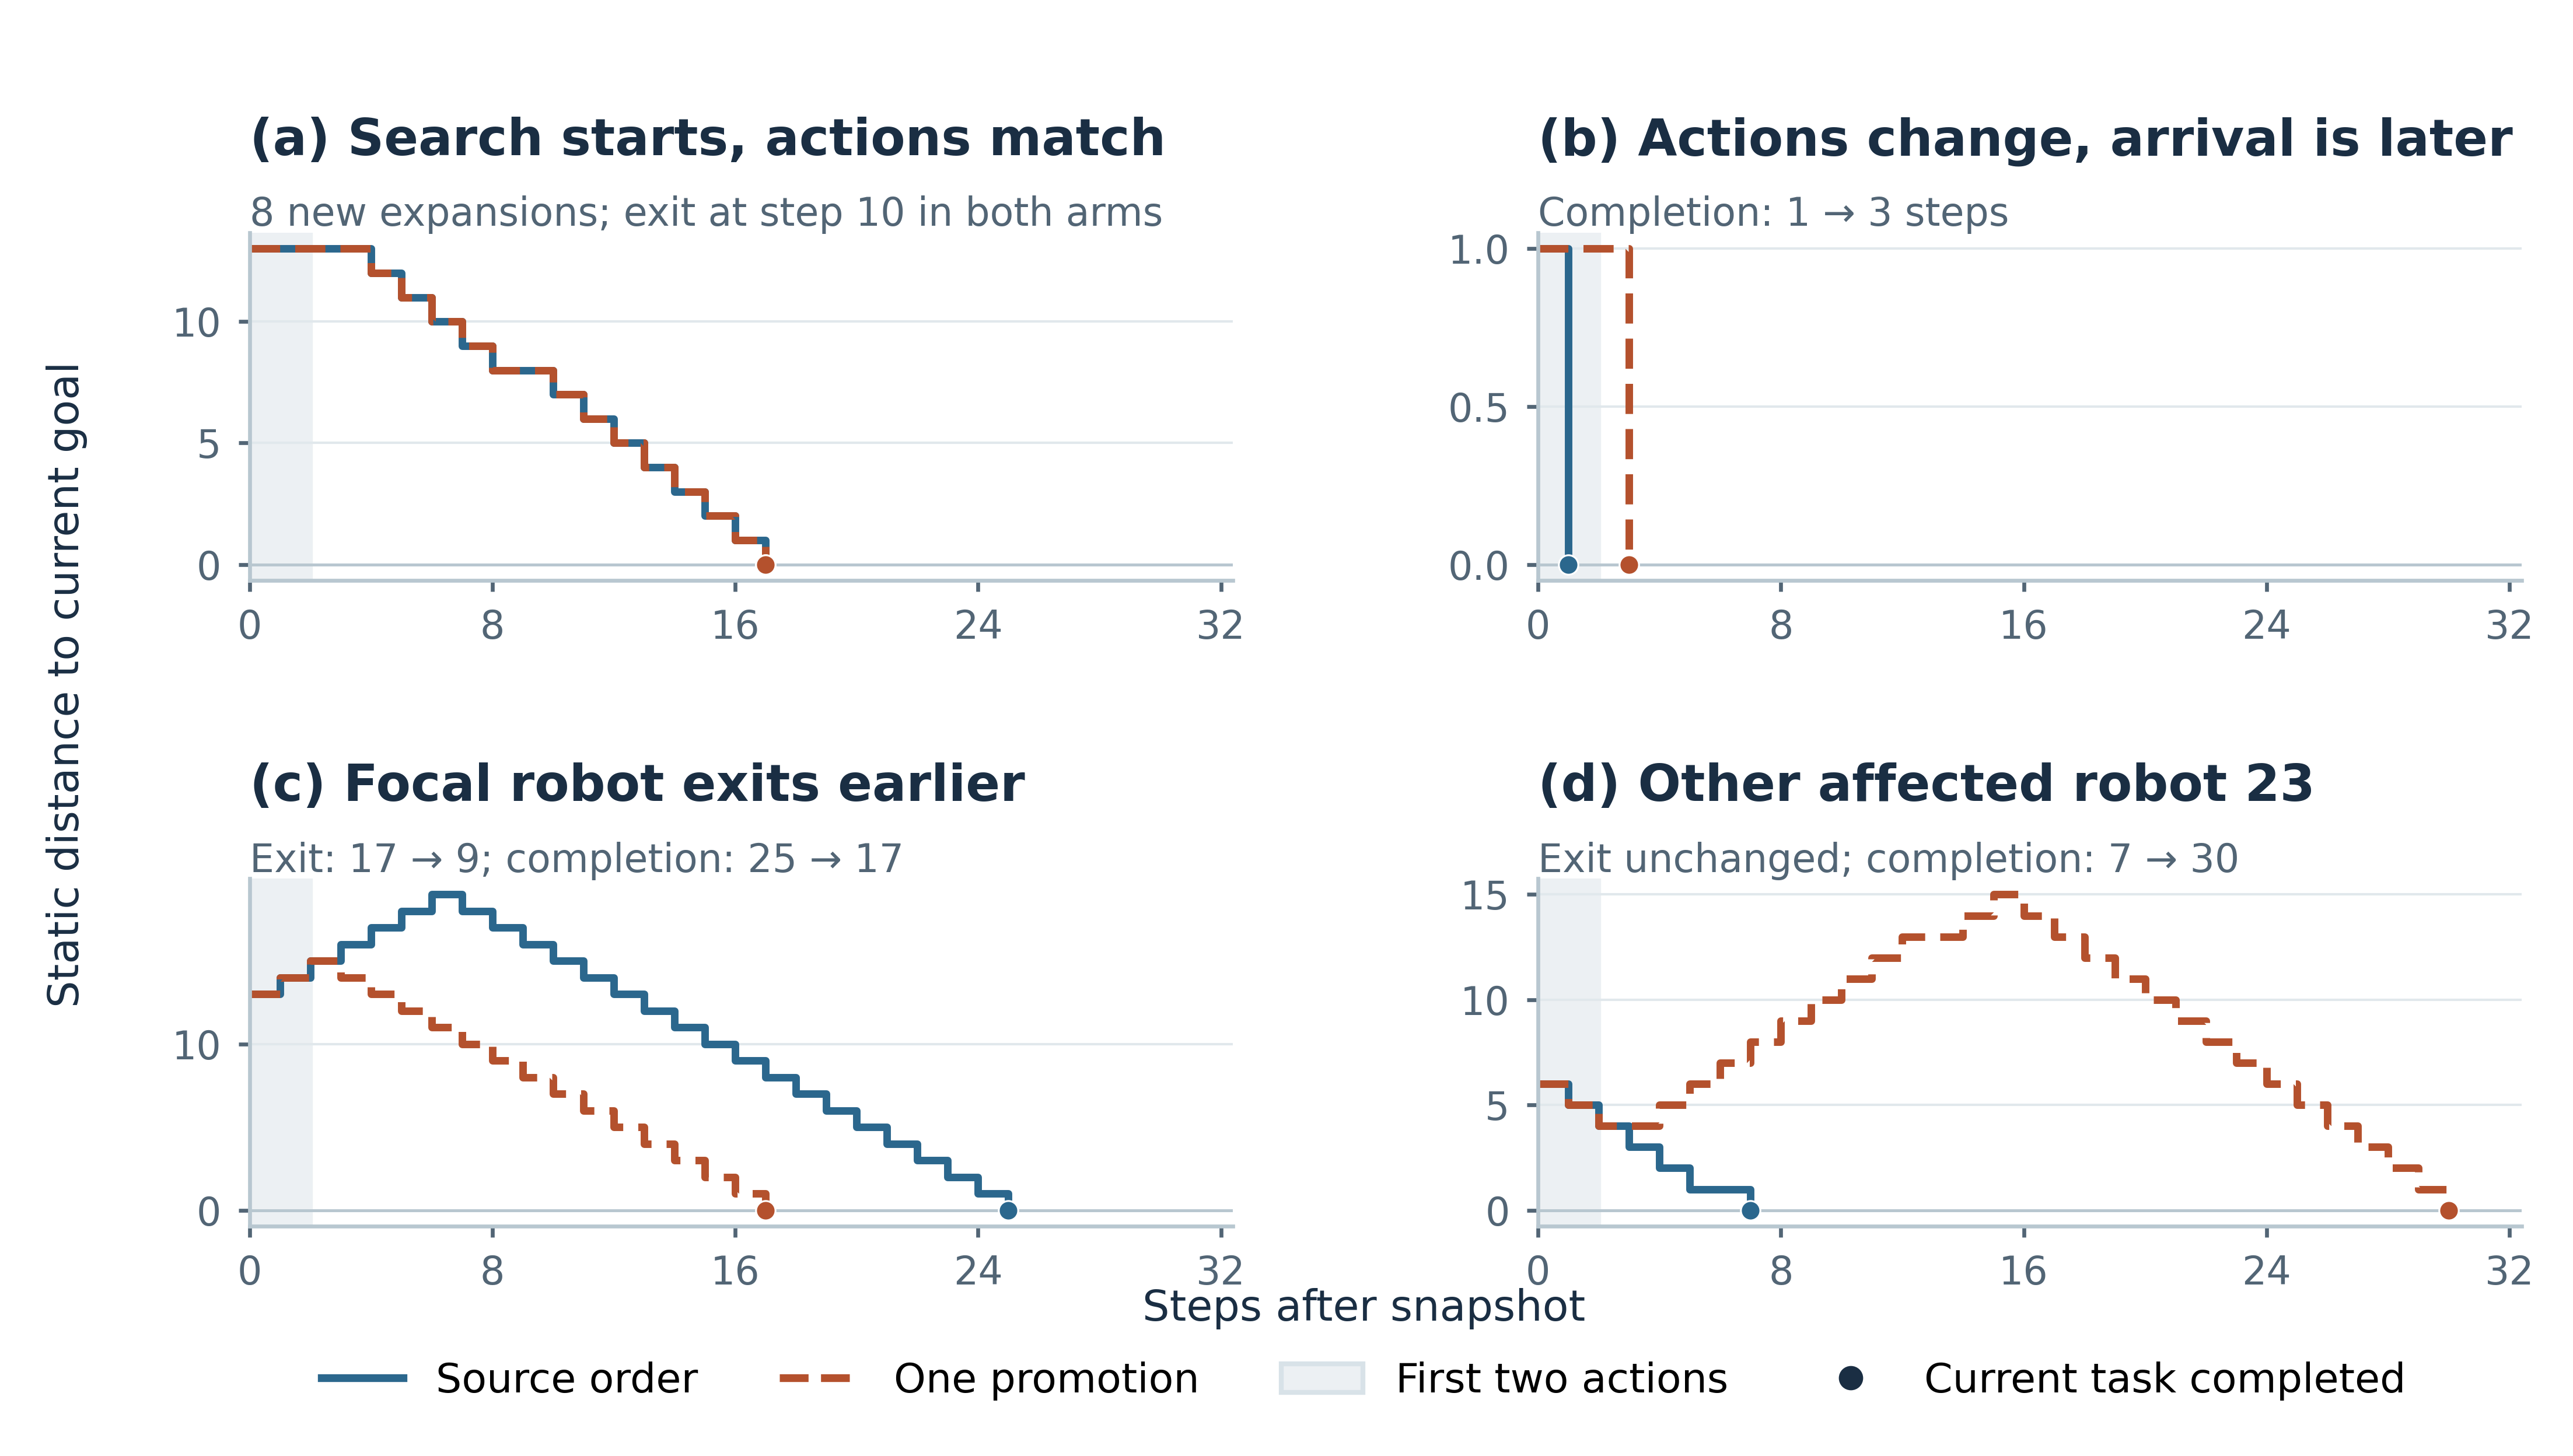
\includegraphics[width=\linewidth,height=.44\textheight,keepaspectratio]{../historical_r4/figures_en/fig5.png}\par
\small\smallskip Figure 5. Static remaining distance in three replayable interventions. Shading marks the first two steps.
\end{minipage}\par\medskip
\subsection*{Section 5.4\quad Matched Conditions and Transfer Across Constructors}\hypertarget{sup:5.4}{}
Restricting the historical cohorts to 24 robots and a congestion source yields E3 in 0/146 overdue and 16/480 exploratory pairs. The focal selection, sampling weights, and seeds still differ. See Appendix \hyperlink{display:TableA1}{Table A1} by map, budget, and rank. The new matched-condition validation excludes 52 of 512 designated times without a focal robot and 15 already ranked first, leaving 445 pairs. The groups with or without nearby opposite-direction traffic have 11/360 and 4/85 E3 cases, a raw difference of \ensuremath{-}1.65 percentage points (scenario interval \ensuremath{-}6.70 to 2.56). Of 12 map \ensuremath{\times} budget \ensuremath{\times} rank cells, 11 have common support, covering 423 pairs. The standardized difference is +0.48 percentage points (\ensuremath{-}2.87 to 3.24). The interval uses the 17,332 of 50,000 resamples retaining common support. Its precision is limited by the sparse group without opposing traffic. A four-cell proximity marker can occur across walls and parallel aisles, so it does not identify competition for the same edge.

\par\medskip\noindent\begin{minipage}{\linewidth}\centering
\hypertarget{display:Figure6}{}%
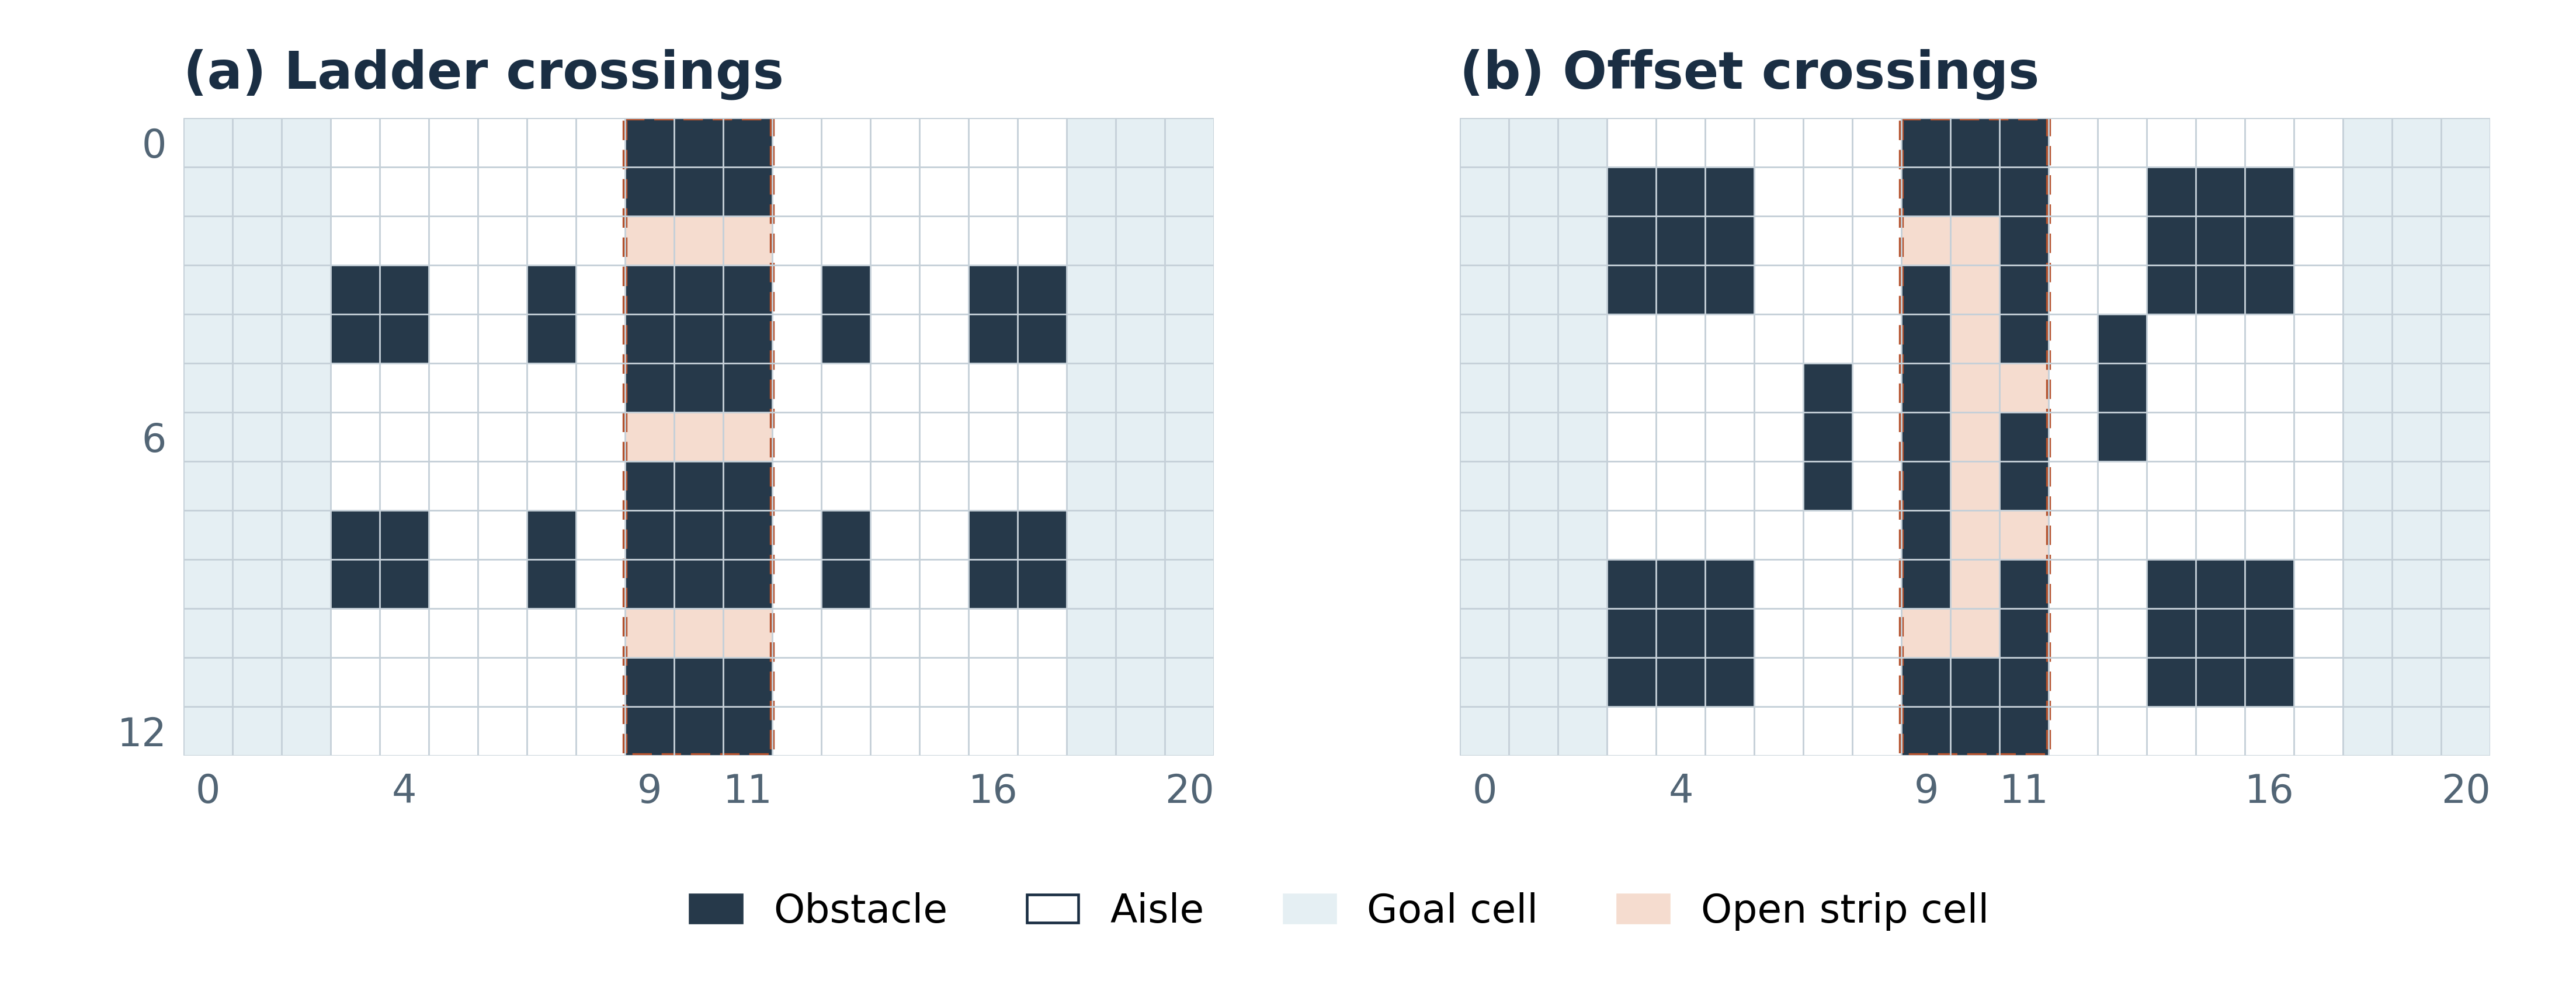
\includegraphics[width=\linewidth,height=.44\textheight,keepaspectratio]{../historical_r4/figures_en/fig6.png}\par
\small\smallskip Figure 6. Two independent warehouse topologies used for transfer tests. The dashed outline marks the strip at x=9--11.
\end{minipage}\par\medskip
\par\medskip\noindent\begin{minipage}{\linewidth}
\small\hypertarget{display:Table8}{}\textbf{Table 8. Replication on new layouts and goal streams}\par\smallskip
\setlength{\tabcolsep}{4pt}\renewcommand{\arraystretch}{1.12}
\begin{tabular}{@{}>{\raggedright\arraybackslash}p{\dimexpr0.13582\linewidth-1.62985\tabcolsep\relax}>{\raggedright\arraybackslash}p{\dimexpr0.11194\linewidth-1.34328\tabcolsep\relax}>{\raggedright\arraybackslash}p{\dimexpr0.17313\linewidth-2.07761\tabcolsep\relax}>{\raggedright\arraybackslash}p{\dimexpr0.12388\linewidth-1.48657\tabcolsep\relax}>{\raggedright\arraybackslash}p{\dimexpr0.10448\linewidth-1.25373\tabcolsep\relax}>{\raggedright\arraybackslash}p{\dimexpr0.17164\linewidth-2.05970\tabcolsep\relax}>{\raggedright\arraybackslash}p{\dimexpr0.17910\linewidth-2.14925\tabcolsep\relax}@{}}
\toprule
\textbf{Layout} & \textbf{Node cap} & \textbf{Constructor} & \textbf{Scenarios} & \textbf{Pairs} & \textbf{E1 / E2 / E3} & \textbf{Source rate} \\
\midrule
Ladder & 120 & Recursive & 12 & 114 & 15 / 0 / 2 & 144.66 \\
Ladder & 120 & Serial & 12 & 180 & 90 / 0 / 0 & 0.52 \\
Ladder & 336 & Recursive & 12 & 109 & 0 / 2 / 2 & 144.27 \\
Ladder & 336 & Serial & 12 & 180 & 15 / 0 / 0 & 1.20 \\
Offset & 120 & Recursive & 12 & 155 & 22 / 4 / 9 & 109.93 \\
Offset & 120 & Serial & 12 & 180 & 61 / 0 / 0 & 0.00 \\
Offset & 336 & Recursive & 12 & 154 & 0 / 2 / 3 & 112.47 \\
Offset & 336 & Serial & 12 & 180 & 0 / 0 / 0 & 0.00 \\
\bottomrule
\end{tabular}
\par\smallskip Source rate is the number of completions per 100 steps from step 65 through 320. Seeds are shared across budgets and constructors on each map.
\end{minipage}\par\medskip
The two source constructors yield 1,252 pairs on the new maps and task streams. Among 532 recursive pairs, E1, E2, and E3 occur 37, 8, and 16 times. Completion by step 32 is 530/532 in the original arm and 529/532 under promotion. There are 166 E1 cases among 720 serial pairs. The serial sources nearly stagnate after warm-up and neither arm's focal robot completes in any pair, so E3 cannot be observed. E2 does not occur either. Appendix \hyperlink{display:TableA3}{Table A3} separates other robots' completion statuses and \hyperlink{display:Table8}{Table 8} reports source throughput. This stress condition shows that new search can occur on a nearly stagnant trajectory.

Changing only the common first-round seed on the same 532 recursive snapshots gives 27 E1 cases in both constructors, 10 in recursive only, and 35 in serial only. The corresponding counts are 0, 8, and 31 for E2 and 2, 14, and 12 for E3. Because the initial scenario and focal robot are shared, these differences reflect how first-round seed construction affects classifications. The diagnosis applies to both constructors, with service outcomes for individual states depending on the actual reservations and candidate acceptance rule.

\subsection*{Section 5.5\quad Independent Validation on Public Layouts}\hypertarget{sup:5.5}{}
\par\medskip\noindent\begin{minipage}{\linewidth}
\small\hypertarget{display:Table10}{}\textbf{Table 10. Independent fixed-reservation reference for query-level mechanisms}\par\smallskip
\setlength{\tabcolsep}{4pt}\renewcommand{\arraystretch}{1.12}
\begin{tabular}{@{}>{\raggedright\arraybackslash}p{\dimexpr0.24030\linewidth-2.40299\tabcolsep\relax}>{\raggedright\arraybackslash}p{\dimexpr0.16716\linewidth-1.67164\tabcolsep\relax}>{\raggedright\arraybackslash}p{\dimexpr0.16716\linewidth-1.67164\tabcolsep\relax}>{\raggedright\arraybackslash}p{\dimexpr0.12836\linewidth-1.28358\tabcolsep\relax}>{\raggedright\arraybackslash}p{\dimexpr0.14776\linewidth-1.47761\tabcolsep\relax}>{\raggedright\arraybackslash}p{\dimexpr0.14925\linewidth-1.49254\tabcolsep\relax}@{}}
\toprule
\textbf{Label} & \textbf{Original positives} & \textbf{Promoted positives} & \textbf{Total} & \textbf{False +} & \textbf{False \ensuremath{-}} \\
\midrule
B \textperiodcentered{} budget & 59 & 0 & 59 & 0 & 0 \\
R \textperiodcentered{} reservations & 87 & 91 & 178 & 0 & 0 \\
G \textperiodcentered{} goal rule & 78 & 78 & 156 & 0 & 0 \\
W \textperiodcentered{} window length & 37 & 36 & 73 & 0 & 0 \\
\bottomrule
\end{tabular}
\par\smallskip The 920 queries include two per pair. Labels can coexist. There are 31 multi-label queries and 3,680 distinct earliest-arrival checks across the four settings.
\end{minipage}\par\medskip
\par\medskip\noindent\begin{minipage}{\linewidth}
\small\hypertarget{display:Table11}{}\textbf{Table 11. Service and promotion outcomes on the public layouts by stratum}\par\smallskip
\setlength{\tabcolsep}{4pt}\renewcommand{\arraystretch}{1.12}
\begin{tabular}{@{}>{\raggedright\arraybackslash}p{\dimexpr0.15821\linewidth-1.89851\tabcolsep\relax}>{\raggedright\arraybackslash}p{\dimexpr0.12687\linewidth-1.52239\tabcolsep\relax}>{\raggedright\arraybackslash}p{\dimexpr0.08358\linewidth-1.00299\tabcolsep\relax}>{\raggedright\arraybackslash}p{\dimexpr0.17313\linewidth-2.07761\tabcolsep\relax}>{\raggedright\arraybackslash}p{\dimexpr0.15672\linewidth-1.88060\tabcolsep\relax}>{\raggedright\arraybackslash}p{\dimexpr0.14925\linewidth-1.79104\tabcolsep\relax}>{\raggedright\arraybackslash}p{\dimexpr0.15224\linewidth-1.82687\tabcolsep\relax}@{}}
\toprule
\textbf{Map \textperiodcentered{} N \textperiodcentered{} cap} & \textbf{Mean rate} & \textbf{Pairs} & \textbf{E1 / E2 / E3} & \textbf{Done, original / promoted} & \textbf{E3 with shared edge} & \textbf{E3 without shared edge} \\
\midrule
W1 \textperiodcentered{} 24 \textperiodcentered{} 144 & 57.39 & 51 & 18 / 5 / 5 & 47 / 47 & 4/32 & 1/19 \\
W1 \textperiodcentered{} 24 \textperiodcentered{} 432 & 61.85 & 60 & 1 / 3 / 1 & 58 / 57 & 1/32 & 0/28 \\
W1 \textperiodcentered{} 48 \textperiodcentered{} 288 & 78.81 & 43 & 19 / 6 / 0 & 38 / 38 & 0/32 & 0/11 \\
W1 \textperiodcentered{} 48 \textperiodcentered{} 864 & 89.55 & 59 & 1 / 1 / 1 & 51 / 50 & 0/32 & 1/27 \\
W2 \textperiodcentered{} 24 \textperiodcentered{} 144 & 83.82 & 61 & 24 / 9 / 9 & 59 / 60 & 9/32 & 0/29 \\
W2 \textperiodcentered{} 24 \textperiodcentered{} 432 & 90.98 & 63 & 8 / 12 / 3 & 62 / 63 & 3/32 & 0/31 \\
W2 \textperiodcentered{} 48 \textperiodcentered{} 288 & 135.42 & 63 & 27 / 8 / 9 & 57 / 62 & 8/32 & 1/31 \\
W2 \textperiodcentered{} 48 \textperiodcentered{} 864 & 144.14 & 60 & 11 / 8 / 2 & 59 / 59 & 1/32 & 1/28 \\
\bottomrule
\end{tabular}
\par\smallskip Each row contains 16 scenarios. Throughput is completions per 100 steps. Finishes exactly at step 32 count as completed. The shared-edge columns use the number of pairs in each group as denominator.
\end{minipage}\par\medskip
\subsection*{Section 5.6\quad Long-Term Ordering and Joint Decision Criteria}\hypertarget{sup:5.6}{}
\par\medskip\noindent\begin{minipage}{\linewidth}
\small\hypertarget{display:Table12}{}\textbf{Table 12. Descriptive results for seven priority orders with equal stratum weights}\par\smallskip
\setlength{\tabcolsep}{4pt}\renewcommand{\arraystretch}{1.12}
\begin{tabular}{@{}>{\raggedright\arraybackslash}p{\dimexpr0.22090\linewidth-2.20896\tabcolsep\relax}>{\raggedright\arraybackslash}p{\dimexpr0.09851\linewidth-0.98507\tabcolsep\relax}>{\raggedright\arraybackslash}p{\dimexpr0.18209\linewidth-1.82090\tabcolsep\relax}>{\raggedright\arraybackslash}p{\dimexpr0.24627\linewidth-2.46269\tabcolsep\relax}>{\raggedright\arraybackslash}p{\dimexpr0.12985\linewidth-1.29851\tabcolsep\relax}>{\raggedright\arraybackslash}p{\dimexpr0.12239\linewidth-1.22388\tabcolsep\relax}@{}}
\toprule
\textbf{Policy} & \textbf{Rate} & \textbf{Overdue \% \ensuremath{\tau}=2/3/4} & \textbf{Robot median [Q1, Q3] \%} & \textbf{Robot max \%} & \textbf{Max. spell} \\
\midrule
Raw age & 74.54 & 4.96 / 0.79 / 0.18 & 0.14 [0.00, 0.83] & 5.73 & 7.72 \\
Fixed & 75.93 & 4.22 / 0.68 / 0.20 & 0.15 [0.04, 0.58] & 5.03 & 6.73 \\
Relative age & 75.27 & 4.07 / 0.62 / 0.18 & 0.05 [0.00, 0.54] & 4.83 & 6.52 \\
Congestion & 75.84 & 3.92 / 0.57 / 0.12 & 0.07 [0.00, 0.51] & 4.43 & 5.98 \\
Remaining distance & 76.95 & 3.73 / 0.48 / 0.14 & 0.07 [0.00, 0.33] & 3.96 & 5.21 \\
Two-stage & 75.83 & 4.01 / 0.58 / 0.14 & 0.10 [0.00, 0.44] & 4.70 & 6.34 \\
Protection + fixed & 76.10 & 4.19 / 0.71 / 0.22 & 0.19 [0.05, 0.55] & 5.13 & 6.87 \\
\bottomrule
\end{tabular}
\par\smallskip Rate is completions per 100 steps. Each stratum has 16 scenarios. Quantiles and longest spells are calculated within each run before aggregation.
\end{minipage}\par\medskip
\par\medskip\noindent\begin{minipage}{\linewidth}
\small\hypertarget{display:Table13}{}\textbf{Table 13. Primary policy comparisons and Bonferroni-adjusted bounds}\par\smallskip
\setlength{\tabcolsep}{4pt}\renewcommand{\arraystretch}{1.12}
\begin{tabular}{@{}>{\raggedright\arraybackslash}p{\dimexpr0.19104\linewidth-2.67463\tabcolsep\relax}>{\raggedright\arraybackslash}p{\dimexpr0.16716\linewidth-2.34030\tabcolsep\relax}>{\raggedright\arraybackslash}p{\dimexpr0.10448\linewidth-1.46269\tabcolsep\relax}>{\raggedright\arraybackslash}p{\dimexpr0.10448\linewidth-1.46269\tabcolsep\relax}>{\raggedright\arraybackslash}p{\dimexpr0.10896\linewidth-1.52537\tabcolsep\relax}>{\raggedright\arraybackslash}p{\dimexpr0.11642\linewidth-1.62985\tabcolsep\relax}>{\raggedright\arraybackslash}p{\dimexpr0.10448\linewidth-1.46269\tabcolsep\relax}>{\raggedright\arraybackslash}p{\dimexpr0.10299\linewidth-1.44179\tabcolsep\relax}@{}}
\toprule
\textbf{Table 13 Layout \textperiodcentered{} N \textperiodcentered{} cap} & \textbf{Baseline} & \textbf{Overdue \ensuremath{\Delta}} & \textbf{Upper U} & \textbf{Rate \ensuremath{\Delta}} & \textbf{Ratio lower L} & \textbf{U/L pass} & \textbf{Joint} \\
\midrule
Single \textperiodcentered{} 12 \textperiodcentered{} 60 & Congestion & +0.007 & +0.036 & 0.00 & 100.00\% & No/Yes & No \\
Single \textperiodcentered{} 12 \textperiodcentered{} 60 & Relative age & \ensuremath{-}0.163 & +0.054 & \ensuremath{-}0.04 & 94.60\% & No/No & No \\
Single \textperiodcentered{} 12 \textperiodcentered{} 168 & Congestion & \ensuremath{-}0.004 & 0.000 & \ensuremath{-}0.04 & 99.61\% & No/Yes & No \\
Single \textperiodcentered{} 12 \textperiodcentered{} 168 & Relative age & +0.033 & +0.170 & \ensuremath{-}0.30 & 94.67\% & No/No & No \\
Single \textperiodcentered{} 24 \textperiodcentered{} 120 & Congestion & +0.013 & +0.675 & \ensuremath{-}0.61 & 95.07\% & No/Yes & No \\
Single \textperiodcentered{} 24 \textperiodcentered{} 120 & Relative age & +0.080 & +1.170 & \ensuremath{-}0.56 & 92.95\% & No/No & No \\
Single \textperiodcentered{} 24 \textperiodcentered{} 336 & Congestion & \ensuremath{-}0.049 & +0.306 & +0.09 & 96.57\% & No/Yes & No \\
Single \textperiodcentered{} 24 \textperiodcentered{} 336 & Relative age & +0.132 & +0.850 & +1.09 & 94.75\% & No/No & No \\
Bypass \textperiodcentered{} 12 \textperiodcentered{} 60 & Congestion & +0.011 & +0.040 & \ensuremath{-}0.04 & 99.66\% & No/Yes & No \\
Bypass \textperiodcentered{} 12 \textperiodcentered{} 60 & Relative age & \ensuremath{-}0.217 & +0.054 & +1.00 & 99.58\% & No/Yes & No \\
Bypass \textperiodcentered{} 12 \textperiodcentered{} 168 & Congestion & 0.000 & 0.000 & 0.00 & 100.00\% & No/Yes & No \\
Bypass \textperiodcentered{} 12 \textperiodcentered{} 168 & Relative age & \ensuremath{-}0.004 & +0.181 & \ensuremath{-}0.22 & 97.37\% & No/Yes & No \\
Bypass \textperiodcentered{} 24 \textperiodcentered{} 120 & Congestion & +0.027 & +0.215 & +0.43 & 99.12\% & No/Yes & No \\
Bypass \textperiodcentered{} 24 \textperiodcentered{} 120 & Relative age & \ensuremath{-}0.143 & +0.251 & +3.08 & 100.45\% & No/Yes & No \\
Bypass \textperiodcentered{} 24 \textperiodcentered{} 336 & Congestion & +0.040 & +0.313 & +0.09 & 98.73\% & No/Yes & No \\
Bypass \textperiodcentered{} 24 \textperiodcentered{} 336 & Relative age & \ensuremath{-}0.085 & +0.278 & +0.48 & 97.49\% & No/Yes & No \\
\bottomrule
\end{tabular}
\par\smallskip Overdue \ensuremath{\Delta} and U are in pp. Rate \ensuremath{\Delta} is per 100 steps. Each stratum has 16 paired scenarios and 50,000 replicates. Nominal confidence per bound is 99.84375\%. U\textless{}0 and L\textgreater{}95\% are required.
\end{minipage}\par\medskip
\par\medskip\noindent\begin{minipage}{\linewidth}\centering
\hypertarget{display:Figure9}{}%
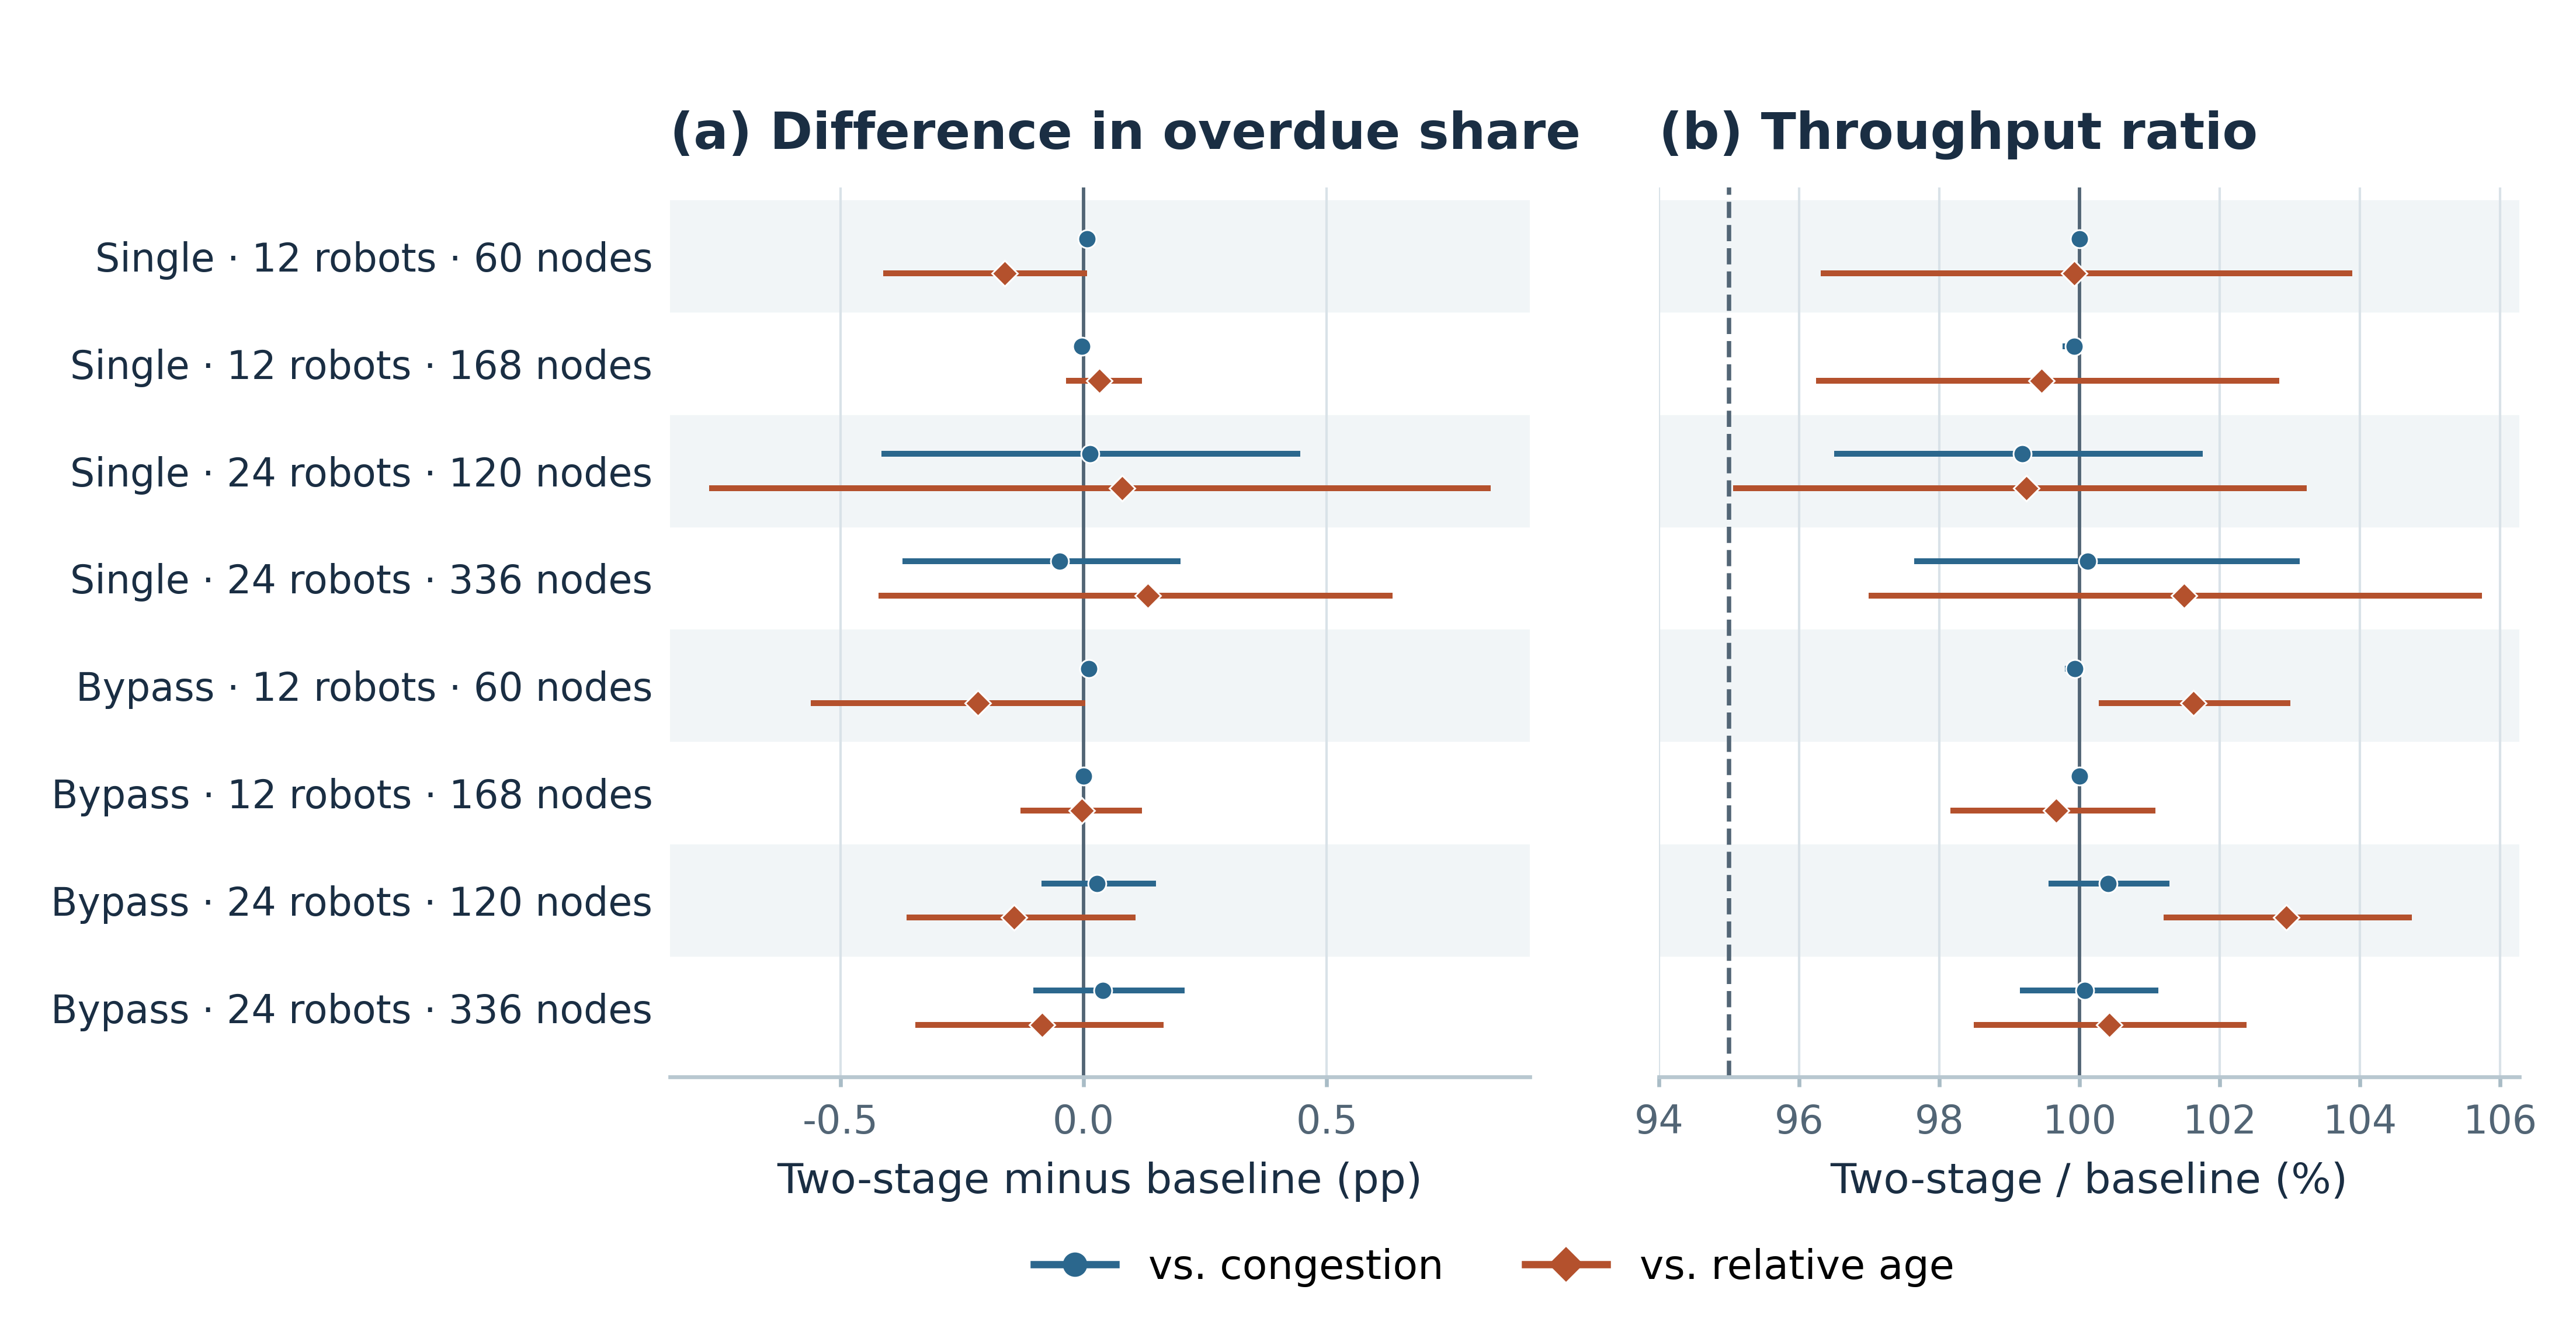
\includegraphics[width=\linewidth,height=.44\textheight,keepaspectratio]{../historical_r4/figures_en/fig7.png}\par
\small\smallskip Figure 9. Effects of two-stage ordering against the two individual rules. Intervals are pointwise two-sided 95\% paired intervals.
\end{minipage}\par\medskip
\end{document}
